\documentclass[twocolumn]{svjour3}

\usepackage{graphicx}
\usepackage[utf8]{inputenc}
\usepackage{listings}
\usepackage{fancyvrb}
\usepackage[usenames]{color}
\usepackage{url}
\usepackage{hyperref}

\usepackage[numbers]{natbib}
%\usepackage[switch]{lineno}

\usepackage{amsmath} % assumes amsmath package installed
\usepackage{amssymb}  % assumes amsmath package installed

\usepackage{eso-pic} %% Background
%\usepackage{floatflt}

\usepackage{enumerate}
\usepackage{paralist} %for inline lists

\usepackage{pseudocode}
\usepackage{alltt}

% fixme notes
\usepackage[draft,footnote,marginclue]{fixme}

\usepackage{subfigure}
%diagrams
\usepackage{tikz}
%\usetikzlibrary{shapes,decorations,trees}
\usetikzlibrary{shapes,trees}

% rotate text in tabular mode
\usepackage{rotating}

%Name of the speaker in a chat
\newcommand{\chatN}[1]{{\footnotesize \textsf{#1}}}
\newcommand{\concept}[1]{{\footnotesize \texttt{#1}}}

\newcommand{\stmt}[1]{{\footnotesize $\langle$\stmttt#1\relax$\rangle$}}
\newcommand{\rawstmt}[1]{{\footnotesize \stmttt#1\relax}}
\def\stmttt#1 #2 #3\relax{{\tt#1} {\bf{\tt #2}} {\tt #3}}

\newcommand{\setstmt}[1]{{\footnotesize [\setstmttt#1\relax]}}
\def\setstmttt#1,#2\relax{\rawstmt{#1}, \rawstmt{#2}}

\newcommand{\ie}{{\textit{i.e.~}}}
\newcommand{\cf}{{\textit{cf~}}}
\newcommand{\eg}{{\textit{e.g.~}}}
% 
% \AddToShipoutPicture{%
%   \AtTextCenter{%
%     \makebox(0,0)[c]{\resizebox{\textwidth}{!}{%
%       \rotatebox{25}{\textsf{\textbf{\textcolor[gray]{0.90}{DRAFT}}}}}}%
%   }%
%  }
 
%------------------------------------------------------------------------- 

\journalname{International Journal of Social Robotics}

\begin{document}
%\linenumbers

\title{Grounding the interaction: anchoring situated discourse in everyday human-robot interaction}

\author{
S\'everin Lemaignan \and
Raquel Ros \and
E. Akin Sisbot \and
Rachid Alami \and
Michael Beetz
}

\institute{ 
	S\'everin Lemaignan \and Raquel Ros \and E. Akin Sisbot \and Rachid Alami
	\at
	CNRS - LAAS, 7 avenue du Colonel Roche, F-31077 Toulouse, France\\
	Université de Toulouse, UPS, INSA, INP, ISAE, LAAS, F-31077 Toulouse, France\\
	\email{\{slemaign, rrosespi, sisbot, rachid\}@laas.fr}
	\and
	S\'everin Lemaignan \and Michael Beetz
	\at
	Intelligent Autonomous Systems, Technische Universität München, Munich, Germany\\
	\email{\{lemaigna, beetz\}@in.tum.de}
}

\maketitle

\begin{abstract}
This paper presents how extraction, representation and use of symbolic
knowledge from real-world perception and human-robot verbal and non-verbal
interaction can actually enable a grounded and shared model of the world that
is suitable for later high-level tasks such as dialogue understanding. We show how
the anchoring process itself relies on the situated nature of human-robot
interactions. We present an implementation, including a specialized symbolic
knowledge representation approach based on Description Logics, and case studies
on several robotic platforms that demonstrate these cognitive capabilities.
\end{abstract}

%%%%%%%%%%%%%%%%%%%%%%%%%%%%%%%%%%%%%%
\section{Grounding human interaction into robot knowledge}

\subsection{Situated speech acts}
\label{intro_example}

A messy table, covered with cardboard boxes, books, video tapes... Thomas is
moving out and is packing everything with the help of Jido, his robot
(Fig.~\ref{fig|vpt}).

``Jido, give me that'', says Thomas while looking at a box that contains a
video tape. The robot smoothly grasps the tape, and hands it to the him.

While this kind of interaction should hopefully sound quite familiar in a
foreseeable future, our robots are not yet quite up to the task, neither
regarding natural language understanding nor plan-making and manipulation.

To be combined together, those abilities require an unambiguous and shared
representation of concepts (objects, agents, actions...) underlying the
interaction: what are the prerequisites for such a sentence --``Jido,
give me that''-- to be understood by the robot, correctly interpreted in the
spatial context of the interaction, and eventually transformed into an action?

Austin~\cite{Austin1962} would have at first glance analyzed this kind of
sentence as a \emph{speech act}, comprising of \emph{locutionary},
\emph{illocutionary} and possibly \emph{perlocutionary} acts. First, we want to
understand the direct meaning of the sentence (\emph{locutionary act}): we must
acquire the sentence, convert it into a useful syntactic form (probably through
speech recognition), and understand the semantics of the sentence, \ie What is
referred by ``\textit{Jido}''? What is ``\textit{give}''? What is
``\textit{me}''? And ``\textit{that}''?

Working in a situated context, we want furthermore to \emph{resolve} these
semantics atoms, \ie ground them in the sensory-motor space of the robot. For
instance, ``\textit{this}'' is a demonstrative pronoun that refers in this
context to the object the human is focusing on (whatever \textit{focusing}
means). In this example Thomas is looking at something, which is a possible
cue. But it could as well be pointing at something or making reference to some
previously mentioned concept. 

\begin{figure}%[!ht] 
	\centering
	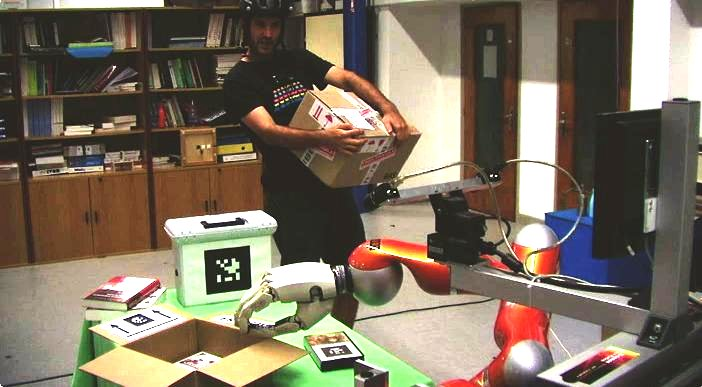
\includegraphics[width=1.0\linewidth]{images/pt.jpg} 
	\caption{Interacting with
	the robot in an everyday setup: the human asks for help in vague terms, the
	robot takes into account the human's spatial perspective to refine its
	understanding of the question.} 
	\label{fig|vpt} 
\end{figure}


Second, the \emph{illocutionary force}, \ie the \emph{intent} of the utterance
as thought by the agent, must be extracted and understood. In our example,
Thomas obviously wants an action to be performed by the robot. The action
parametrization is conveyed by the semantics attached to the words and the
grammatical structure of the sentence. In our example, the type of action is
given by the verb ``\textit{give}''. Assuming the robot has some procedural
knowledge attached to this symbol, the action type can be considered as
grounded for the robot. We can as well understand that the recipient of the
action is the human, the performer is the robot itself, and the object acted
upon is the tape. These are the basic \emph{thematic roles}~\cite{Gruber1965}
that can be extracted from the sentence that allow for fully grounding the action
\footnote{The third class of speech acts, the \emph{perlocutionary acts}, deal
with implicit speaker's expectations. We will not consider it further in this
article}.

%Finally, the implicit speaker's expectation can sometimes be conveyed --the
%\emph{perlocutionary act}-- and should be taken into account. If Thomas would
%have said instead ``Jido, this box is too heavy for me'', he may implicitly
%expect the robot to memorize the fact that the box's weight is over his
%capabilities, and it may as well imply that Thomas is requiring help to carry
%the box.

\subsection{Approach}

Extracting these speech acts and turning them into content processable by the
robot is a difficult challenge in the general case. We base our approach on
three distinct, inter-related cognitive functions.
Figure~\ref{fig|overall-process} illustrates the general context, while
Figure~\ref{fig|main-components} summarizes the interactions between the three
main components:

\begin{inparaenum}[\itshape 1)]

\item \emph{Physical environment modeling} and \emph{spatial reasoning}
(grouped under the term \emph{situation assessment}): these components are in
charge of building and maintaining a coherent model of the physical world. This
model is realistic in the sense that it relies on accurate 3D models of both
manipulated objects and humans. It also has dedicated mechanisms to manage
disappearing or occluded objects.  The geometric model is used to compute
several spatial properties of the scene that actually convert the original
sensory data into symbolic beliefs, including relative locations of objects,
visibility state, gestures (such as pointing), etc.  Assuming that other agents
are also represented in the model, the same computations are applied to analyze
the scene from each agent's point of view (\ie from their \emph{perspectives}).

\item \emph{Knowledge representation and management}: the robot is endowed with
an active knowledge base that provides a logically sound symbolic model of its
beliefs of the world, as well as models for each cognitive agent the robot
interacts with. Each of these models is independent and logically consistent,
enabling reasoning on different perspectives of the world that would otherwise
be considered inconsistent (for instance, an object can be visible for the
robot but not for the human. This object can have at the same time the property
\concept{isVisible \textbf{true}} and \concept{isVisible \textbf{false}} using
two different models).  Our platform relies on OWL-DL\footnote{\emph{Web
Ontology Language - Description Logics}, a decidable subset of the first-order
logics, \url{http://www.w3.org/TR/owl2-primer/}} ontologies and features
continuous storage, querying and event triggering over the pool of facts known
by the robot.

Used in combination with the situation assessment framework, the robot is thus
able to maintain different symbolic models of the world, one per agent. This
proves an essential feature (\cite{Roy2005,Kruijff2010}) to enable
perspective-aware grounding of natural language as we will see in next
sections.


\item \emph{Dialogue input processing}: a subsystem which includes natural
language parsing capabilities, disambiguation routines and interactive concept
anchoring. We focused our efforts on three classes of utterances commonly found
in human-robot interaction: \emph{statements} (\ie new facts the human wants to
inform the robot), \emph{orders} (or more generically \emph{desires}) and
\emph{questions on declarative knowledge} (whose answers do not require
explicit planning). This would roughly cover the \emph{representative}
(sometimes referred as \emph{assertive}) and \emph{directive} illocutionary
acts in Searle's~\cite{Searle1976} classification.

\end{inparaenum}

Based on these three components we have developed several grounding mechanisms
for situated verbal interaction and integrated them into a broader control
architecture for indoor service robots. 

\begin{figure}[!ht]
\centering
  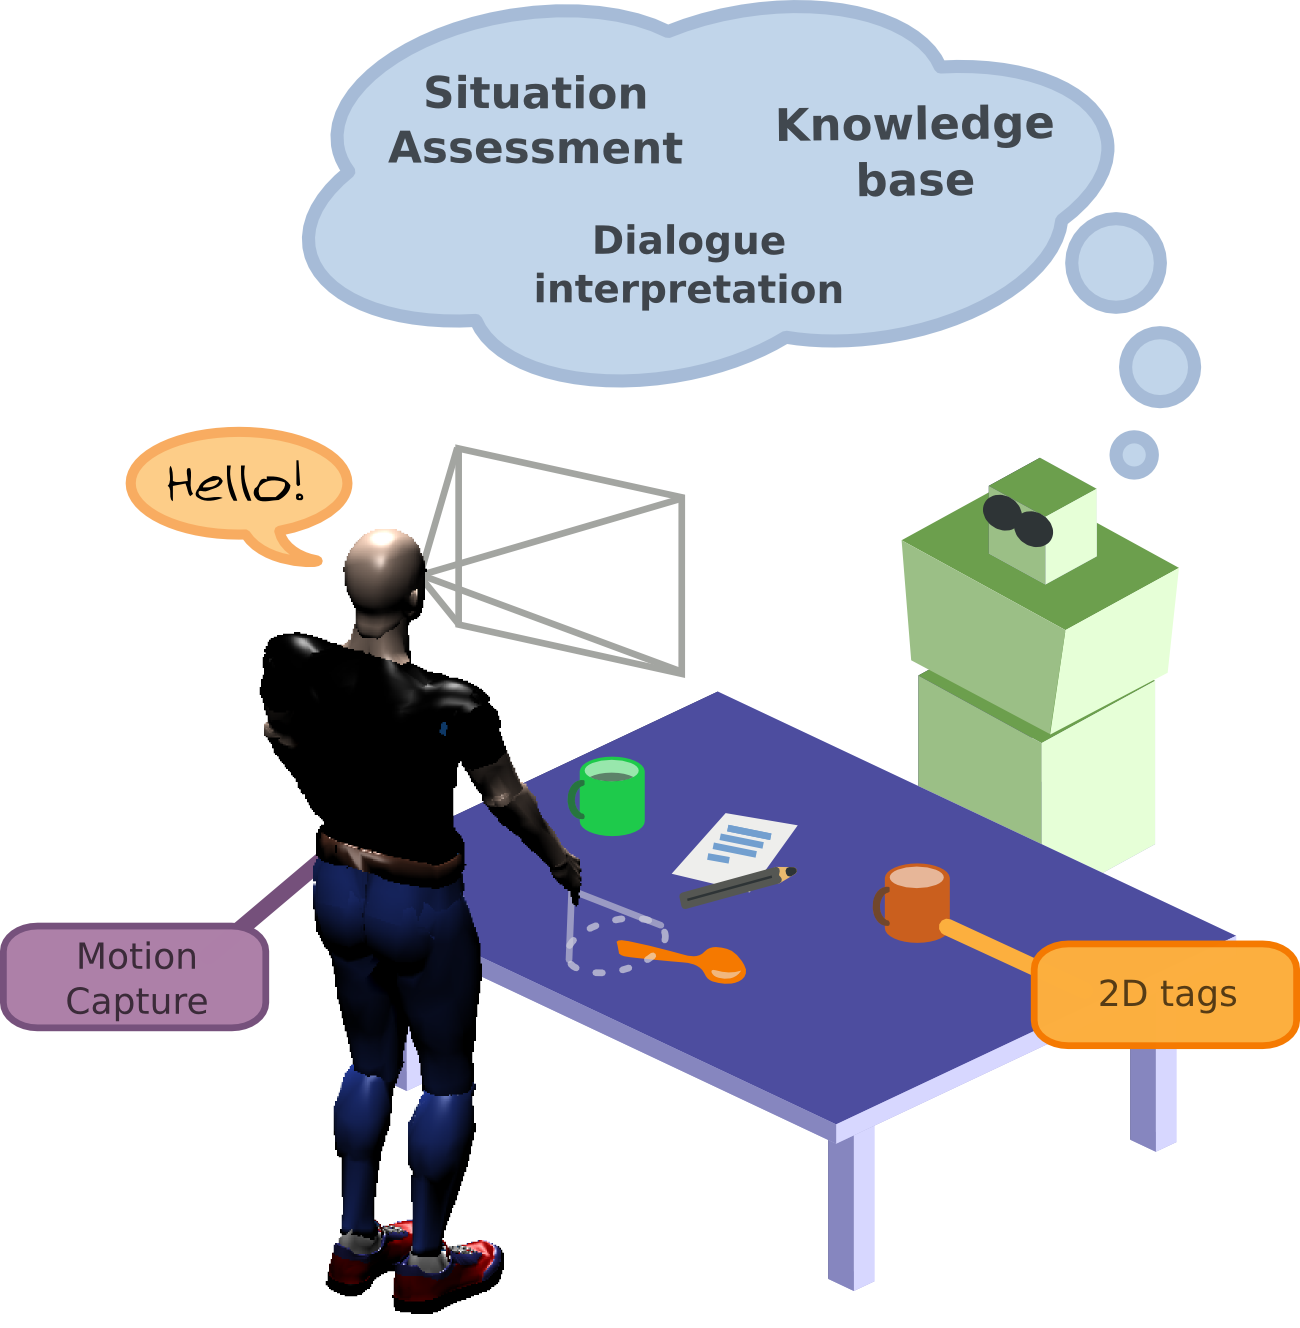
\includegraphics[width=0.8\linewidth]{images/grounding_robot.png}
  \caption{Generic model of cognitive abilities interactions for grounding}
  \label{fig|overall-process}
\end{figure}

\begin{figure}[!ht]
\centering
  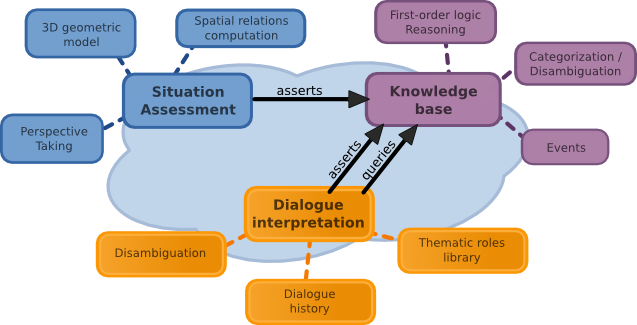
\includegraphics[width=0.9\linewidth]{images/grounding.png}
  \caption{The three main components of our architecture and their connections. Submodules are presented in subsequent sections.}
  \label{fig|main-components}
\end{figure}

%~ The system we describe here relies on two distinct activities that run concurrently and continuously: maintenance of a symbolic model from real world interpretation on one hand, and verbal interaction with agents on the other hand.
%~ 
%~ The first activity consists in two main steps:
%~ 
%~ \renewcommand{\labelenumi}{(\alph{enumi})}
%~ \begin{enumerate}
%~ \item The \emph{Object Identification} step is expected to provide consistent identification of objects in the environment. It does not involve any semantic functionality like automatic labelling, classification or annotation capabilities. It is in charge of solving what is merely a perception issue related to the ability to assign some identifier consistently. This is in the general case an open research issue that is outside of the scope of this paper. In our experiments, we will use simplified approaches (like tag-based object identification and motion capture).
%~ 
%~ Besides identification, other perceptual informations are extracted at this step, such as absolute size, color, and more importantly, its spatial position relative to the robot.
%~ 
%~ \item \emph{Physical environment modeling} and \emph{spatial reasoning} are then in charge of rebuilding a coherent physical model of the world based on information extracted in the first step. Once available, the geometric model is used to compute several spatial properties of the scene that actually convert the original sensory data into symbolic beliefs. This includes relative locations of objects, visibility state, gestures like pointing, etc. Assuming that other agents are as well represented in the model, the same computations can be applied to analyze the scene from each agents' point of view (\ie from their \emph{perspectives}).
%~ \end{enumerate}
%~ 
%~ The output of this second step needs to be stored for later reuse: we introduce to that end a general-purpose knowledge management system that relies on a sound logical system (the Description Logics) to store, manipulate and reason about symbolic knowledge. This system is described at length in the next section.
%~ 
%~ The verbal interaction activity relies on three main steps:
%~ 
%~ \begin{enumerate}
%~ \item The \emph{parsing} of natural language aimed at extracting grammatical structures from a sentence,
%~ 
%~ \item The \emph{resolution} of concepts, where words used by the user are associated with the underlying concept they represent, as stored in the robot knowledge base. This step may require an additional interactive disambiguation step if the robot can not successfully bind a word to the concept it represents.
%~ 
%~ \item Finally, the \emph{content analysis} step extracts the \emph{intention} of the sentence and handles it. Orders, questions, statements (new information) are separately processed.
%~ \end{enumerate}

\subsection{Related work}

Our work builds on top of years of work in the artificial intelligence
community around the symbol grounding issue: we can mention
Searle~\cite{Searle1980} who introduces it with the \emph{Chinese room}
metaphor, Harnard~\cite{Harnad1990} who coins the following (slightly
paraphrased in the robotic context) definition of symbol grounding:
\emph{``make the meanings of the meaningless symbol tokens intrinsic to the
robotic system"}, Coradeschi and Saffioti~\cite{Coradeschi2003} who focus on
robotics and define the meaning of \emph{anchoring} as \emph{``the process of
creating and maintaining the correspondence between symbols and sensor data
that refer to the same physical object''}, Ziemke~\cite{Ziemke1999} who
elaborates on the need of embodiment for symbol grounding, and
Sloman~\cite{Sloman2007} who criticizes the \emph{``concept empricism"} that
underlies symbol grounding.

Our contribution relates to two narrower fields: natural language in embodied
interaction contexts and knowledge building and representation in robotic
systems.

Processing natural language in situated contexts is already an established
research field. In~\cite{Roy2005}, Roy and Reiter summarize what they see as
the main challenges to be tackled: cross-modal representation systems,
association of words with perceptual and action categories, modeling of
context, figuring out the right granularity of models, integrating temporal
modeling and planning, ability to match past (learned) experiences with the
current interaction and ability to take into account the human perspective.
This list offers an interesting entry point to evaluate our contribution.

Kruijff et al. provides in~\cite{Kruijff2010} an up-to-date survey of
literature on situated human-robot dialogue, focusing on formal representation
systems, bi-directionality of the interaction and context building. They point
out as well that compared to the cognitive psychology community, the ``situated
AI'' community started only recently to take into account agents' focus of
attention, perspective and temporal projection abilities.

Dialogue processing in real robots have been explored by several teams.  Brick
and Scheutz~\cite{Brick2007} have contributions regarding natural language
processing in an incremental way, and how this enables instant back-channel
feedback (like nodding). Hüwel et al.~\cite{Huwel2006} propose the concept of
\textit{Situated Semantic Unit}: atoms are extracted from sentences exposing
semantic links to other units. The parser tries to satisfy these links and
rates the semantic interpretation of the sentence. Used in conjunction with
ontologies, their approach offers robustness to ungrammatical or partial
utterances. They validated the approach with an extensive user-study.

Zender et al.~\cite{Zender2009} address the generation of referring expressions
(\emph{GRE}) in situated dialogue for topological knowledge.  They consider
both the reference resolution and reference description tasks, and rely on
OWL-DL representation and SPARQL\footnote{{\em SPARQL Protocol and RDF Query
Language}, \url{http://www.w3.org/TR/rdf-sparql-query/}} to extract
\emph{topological contexts} from their knowledge base.

While mostly implemented on virtual agents, the GLAIR cognitive architecture by
Shapiro and Bona~\cite{Shapiro2009} is an architecture explicitly built to
tackle the grounding issue from the percept to the decision. It is a
three-layers architecture: a \emph{Knowledge Layer}, a low-level
\emph{Sensori-Actuator Layer} and an intermediate \emph{Perceptuo-Motor Layer}
that binds the previous two.  The knowledge layer relies on a custom knowledge
representation language (more expressive than first-order logic), and natural
language processing capabilities similar to ours are available. The GLAIR
project has been only demonstrated in a limited set of environments, but
exhibits interesting features such as explicit management of contexts of facts
and memory models (long term/short term, episodic/semantic).

Also worth mentioning, Mavridis and Roy~\cite{Mavridis2005} propose the idea of
a \emph{grounded situation model} which is an amodal model of the world where
different sensing modalities, including verbal ones (the robot is able to
\emph{imagine} objects), are merged. Their framework also allows the management of
the interaction history (the human can ask for a past event). They propose an
implementation in an environment built on simple entities (a manipulator arm
and colored balls).

In the field of symbolic knowledge processing for robots, Gunderson and
Gunderson~\cite{Gunderson2008} introduce the concept of \emph{reification}
(based on both recognition and pre-afference) as an intermediate step between
pattern recognition and symbol grounding. Their underlying storage of knowledge
relies on ontologies and bio-inspired memory models. While sharing similar
foundations to our work, their proposal is based on fairly simple perceptual
modalities and does not develop complex symbolic models that could enable
human-robot interaction.

Suh et al.~\cite{Suh2007} develop {\sc OMRKF}, an ontology-based reasoning
framework for robotics. They tackle the grounding problem by storing low-level
facts (like SIFT visual features) in a layered symbolic architecture that works
well in simple sensori-motor spaces. However this approach raises concerns
regarding scalability and management of more complex entities or interactions.

Daoutis et al.~\cite{Daoutis2009} introduce one of the first complete
architectures for grounded human-robot interaction. They successfully bind
low-level percepts (including view-point independent SIFT based object
recognition) to a high-level knowledge representation and reasoning system via
a dedicated anchoring module. They base their knowledge model directly on the
\textit{ResearchCyc} ontology (including the \textit{MicroTheories} concept),
used in combination with the CycL language. This enables second-order
logic modeling and access to a large common-sense knowledge base.

Beetz et al.~\cite{Beetz2010} proposes a cognitive architecture called
\textsc{CRAM} (Cognitive Robot Abstract Machine) that integrates
\textsc{KnowRob}~\cite{Tenorth2009a}, a knowledge processing framework based on
Prolog. Its underlying storage is based on an OWL ontology, derived from
\textsc{OpenCyc}. \textsc{CRAM} and \textsc{KownRob} have been demonstrated on
several real-world scenarios, where natural language recipes extracted from
Internet had to be translated into plans and executed in a kitchen environment,
perceived and rebuilt on-line by the robots. While Prolog offers more flexible
modeling (no constraints on the arity of predicate, where Description Logics as
used in our work are limited to binary predicates), it is based on the closed
world assumption (if something cannot be inferred to be true, it is inferred to
be false) whereas we rely on the open world assumption, which is more realistic
in real world scenarios. A probabilistic extension of \textsc{KnowRob}, called
\textsc{ProbCog}~\cite{Jain2009} is also available. While in principle
possible, currently the CRAM architecture does not provide explicit support for
interacting with humans.


\subsection{Contributions}

Besides proposing a new integration model for sensor data, natural language and
symbolic knowledge repositories, our work extends these previous contributions
by tackling more realistic human-robot interactions: open speech; complex,
dynamic, partially unknown human environments; and fully embodied (with arms,
head, ability to move,...) autonomous robots that can perform manipulation.

Four specific contributions are presented in this work: first, we introduce a
novel and versatile knowledge base that models in a formal framework, based on
first-order logics, not only the robot's own beliefs but also every other
cognitive agent the robot interacts with.  This explicit modeling of other
agents' belief states is used for the interaction and eases the implementation
of various advanced cognitive behaviors like learning new concepts or
interactive object discrimination.

Second, we have implemented a framework to extract symbolic facts from complex
real scenes. It is based on a 3D model of the world that the robot builds
on-line by merging different sensor modalities. It computes spatial relations
between perceived objects in real-time and it allows for virtually \emph{viewing}
of the same scene from different points of view, enabling \emph{visual} and
\emph{spatial agent perspective taking}.

Third, the same symbolic knowledge base enables richer language capabilities
for the robot.  We propose a new approach to natural language grounding that is
robust, situated and more generic than what can be found in previous work
on situated language grounding. We present several examples that include
generic recognition and semantic validation of thematic roles (\ie the
semantic roles played by the different nominal groups around a verb), which
can be translated into input for a symbolic task planner, or disambiguation
based on attention foci.

Lastly, our architecture moves away from standard layered approaches. The way
our different components interact together is not easily represented as a
layered architecture because interactions among components are mostly
bidirectional.  This is especially visible for the dialogue input processing:
this component does not simply act as an alternative perceptual input to the
symbolic database, but also actively queries previously acquired knowledge to
disambiguate and validate the newly created symbolic knowledge. This behaviour
leads us to the idea of \emph{knowledge-oriented architecture}, which is
detailed later on.

These points highlight some original aspects of a larger cognitive architecture
that has been deployed and tested on three distinct robotic platforms
(including both humanoid robots and service robots), demonstrating the
versatility and hardware-agnosticism of these developments.

\subsection{Article overview}

In the next section we present in depth the so-called {\sc ORO}
(\emph{OpenRobots Ontology} server) knowledge base, a dynamic knowledge
representation system based on Description Logics ontologies and relying on the
\emph{Open World Assumption}. We present it first, along with its objectives,
since it is the knowledge \textit{hub} of the system, used pervasively by other
components.

Section 3 presents {\sc SPARK} (for \emph{SPAtial Reasoning \& Knowledge}), a
module that merges perceptual information with a coherent geometric model and
builds a symbolic interpretation of the world from the robot's point of view,
as well as an individual symbolic model for each agent currently present in the
environment. 

Section 4 covers in detail the dialogue processing component. The main
algorithms for natural language grounding are described, as well as the
interactions between these component and the knowledge base.

Section 5 presents three use-cases that were conducted on two different
robotic platforms: the \emph{Naming} experiment, where a robot anchors new
knowledge in its model through verbal interaction; the \emph{Spy Game}, where
either the user or the robot tries to guess which object the other player is
thinking of; and a more complex experiment situated in an everyday setup, where
the robot builds models for several agents and interacts with the users using
this knowledge.

%%%%%%%%%%%%%%%%%%%%%%%%%%%%%%%%%%%%%%
\section{ORO, a knowledge management platform} \label{cognitivekernel}

\subsection{On knowledge representation} \label{knowledge_representation}

While \emph{knowledge} has no general definition that researchers agree on, for
our own purposes we define knowledge as \emph{information interpreted in the
cultural and social context of the robot}, where information is a
\emph{statement} or an \emph{assertion} about the world\footnote{In this paper,
statements are always triples \texttt{<subject, predicate, object>}, following
the Description Logics formalism.}. In practical terms, knowledge is made of
statements that are \emph{contextualized}, if possible \emph{synthesized}, and
\emph{limited} to a domain of validity.

These three features have important consequences for the way a knowledge
representation and storage system must be designed. Let us examine them:

\paragraph{Contextualizing} is the ability for a cognitive system to connect a
fact with a \emph{cultural context}, an \emph{interpretive scope} and the set
of other facts previously acquired by the agent.
%~ Since machines are limited to syntactic (in contrast to semantic)
%processing, we are mostly looking for a syntactic (\ie, based on symbols)
%matching between concepts representations (in our case, sets of alphanumeric
%characters).\fxfatal{il faut sans doute évoquer ici la relation
%sémantique/syntactique que propose Choamsky}.

We call \textit{cultural context} a broad set of common, general facts that are
considered widely accepted among the interactors (\eg ``bottles may contain
water''). This knowledge is often referred as \emph{common-sense knowledge}.

By \emph{interpretive scope} we mean that a concept may have different
interpretations depending on the agent, the current situation or the time frame
the statement belongs to. Since a fact in one scope can be different (or even
inconsistent) with a fact in another scope (for instance, one object can be
visible for the robot and invisible for another agent), the underlying
knowledge representation system must properly handle these interpretive
frameworks.

Note that the focus of the ORO platform is on enabling such context to be
effectively represented rather than actually identifying the current context.
While several approaches for building contextualized knowledge are proposed in this
paper (symbolic environment interpretation, perspective taking, grounded
natural language resolution, self-awareness of its own activity), much remains
to be done for a robot to actually identify its current context as well as
contexts that may be referred to.

\paragraph{Synthesis} corresponds to the identification of facts and their
components (concepts and predicates) with respect to other facts. For instance,
if the robot observes a human sitting down at a table, and at the same time, we
tell it that ``Peter is sitting at the table'', we would like the robot to
infer that ``Peter'' may be the name of the human. \textit{Synthesis}
refers to the fact that several, \textit{a priori} uncorrelated, facts
must be associated with the same common concept. This process requires the
ability to control the logical consistency of the knowledge corpus. To
continue with the previous example,  if we add the fact that the human that
is sitting is a woman, the synthesis ``Peter is the name of the human'' is
not valid anymore.

\paragraph{Domain of validity}: its main role is to specify the scope in which
 information is (believed to be) true. It covers several aspects: temporal,
situational and probabilistic. While related to the previous concept of
\emph{interpretive scopes}, the domain of validity addresses the question
whether a fact must be or not considered in a given context. This validity
limitation is not usually carried by the fact itself. In the previous example,
for instance, the robot observes a human sitting at a table.  The fact ``a
human is sitting at the table'' is true only for a limited period of time,
until the human stands up. This period of time is not directly accessible
(the robot does not know how long the human plans to stay), but the
knowledge representation must be able to deal with this uncertainty and
should explicitly label this fact as being limited in time.
%~ ~ To know if a fact is permanent or transitional (as defined by Pollock
%\fxfatal{citation de Langage et Cognition, page 50}) is difficult (especially
%considering that a feature may be considered as permanent or not depending of
%the context: within the situation ``a familly meal''\fxfatal{Check
%translation!}, the fact ``the human is sitting at the table'' could be
%considered as permanent. Conversely, ``ground is static'' is generally
%considered as a static fact, expect if we are talking of planetary mechanics
%for instance. The difficulty lies in the selection of the relevant situation
%in which reasoning must be carried out at a given time) and have currently to
%be defined in the cultural background of the robot.

These three aspects lead us to envisage a knowledge representation system
characterized by the following abilities: 
\begin{itemize}
	\item represent raw information,
	\item render a general cultural background, in the form of common-sense knowledge,
	\item attach interpretive scopes to new statements,
	\item add and connect new statements to knowledge already present,
	\item store restrictions on the domain of validity of the knowledge.
\end{itemize}

Besides, the following active processes would be desirable:
\begin{itemize}
	\item acquire and maintain knowledge perceived from the physical world or
	retrieved from other sources (interaction with other agents, web-based contents,...)
	\item synthesize facts as much as possible,
	\item monitor contexts and accordingly manage the validity of the stored knowledge,
	\item ensure the logical consistency of the knowledge repository, and
	explicit inconsistencies when required\footnote{One may argue that the real world is 
	inherently inconsistent. In this article, we make a
	\textit{consistent world} assumption, in order to leverage reasoning
	capabilities of the first-order logics. This is supported by the natural
	tendency of humans themselves to provide a consistent explanation of their
	world.}.
\end{itemize}

This list does not cover all the possible features that could be exposed by a
symbolic knowledge management system. Bio-inspired memory management (the
ability to forget or reinforce knowledge) or curiosity (the ability to
identify lacking knowledge and actively trigger behaviors to acquire
it\fixme{cite Howa}), to give some examples, could arguably be added to the
list. However, this first analysis sets a convenient reference frame to
understand and evaluate knowledge representation systems, including the
\textsc{ORO} knowledge management system we propose.

\begin{figure}[!ht]
\centering
  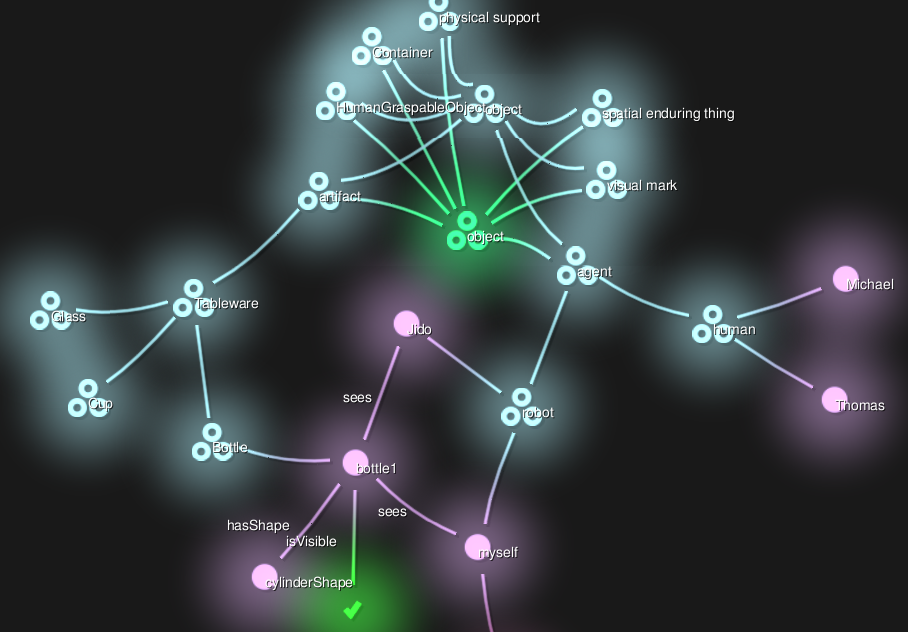
\includegraphics[width=\columnwidth]{images/snapshot_oroview.png}
  \caption{Live snapshot from the \emph{oro-view} viewer depicting the
  knowledge model of the robot during an experiment. Dots represent
  instances (ABox), while circles pyramids are classes (TBox)}
  \label{fig|oro-view}
\end{figure}

\subsection{ORO Architecture}

The ORO platform~\cite{Lemaignan2010} is primarily designed as a central
knowledge storage service implemented as a server where the robot
components can add or query statements at run-time. Figure~\ref{fig|oro-overview}
illustrates the overall architecture. The \emph{front-end} accepts and manages
connections from client components. The clients' requests are processed by a
set of internal modules: basic operations on statements, but also higher
cognitive and human-robot interaction related functionalities are available
(detailed thereafter). External plugins can also be easily added. The modules
rely on several parallel ontology \emph{back-ends} where the knowledge is
actually stored.

Knowledge is represented in ORO in the Description Logics formalism (using the
OWL-DL -- \emph{Web Ontology Language - Description Logics} -- language), as
RDF (\emph{Resource Description Framework}) triples (for instance \stmt{robot
isIn kitchen}). We use the Jena\footnote{\url{http://jena.sourceforge.net/}}
framework as the underlying library to load and build in-memory OWL model. We
use it in conjunction with the
Pellet\footnote{\url{http://clarkparsia.com/pellet/}} reasoner to ensure the
continuous classification of the OWL concept graph: at run-time, newly added
statements are continuously reasoned about (\emph{classified}), and at any time,
the server expose a complete set of statements, both the asserted ones and the
inferred ones. For instance, if \stmt{socrates type Human} and \stmt{Human
subClassOf Mortal} are asserted, the server transparently adds the inferred
statement \stmt{socrates type Mortal}, and a later query retrieving all mortal
entities would return \concept{socrates} as well. The language of the OWL
family use the \emph{Open World Assumption} (if a fact can not be inferred as
true, it does not mean that it is inferred to be false), and the Pellet
reasoner honors this assumption as well.

\begin{figure}[!ht]
\centering
  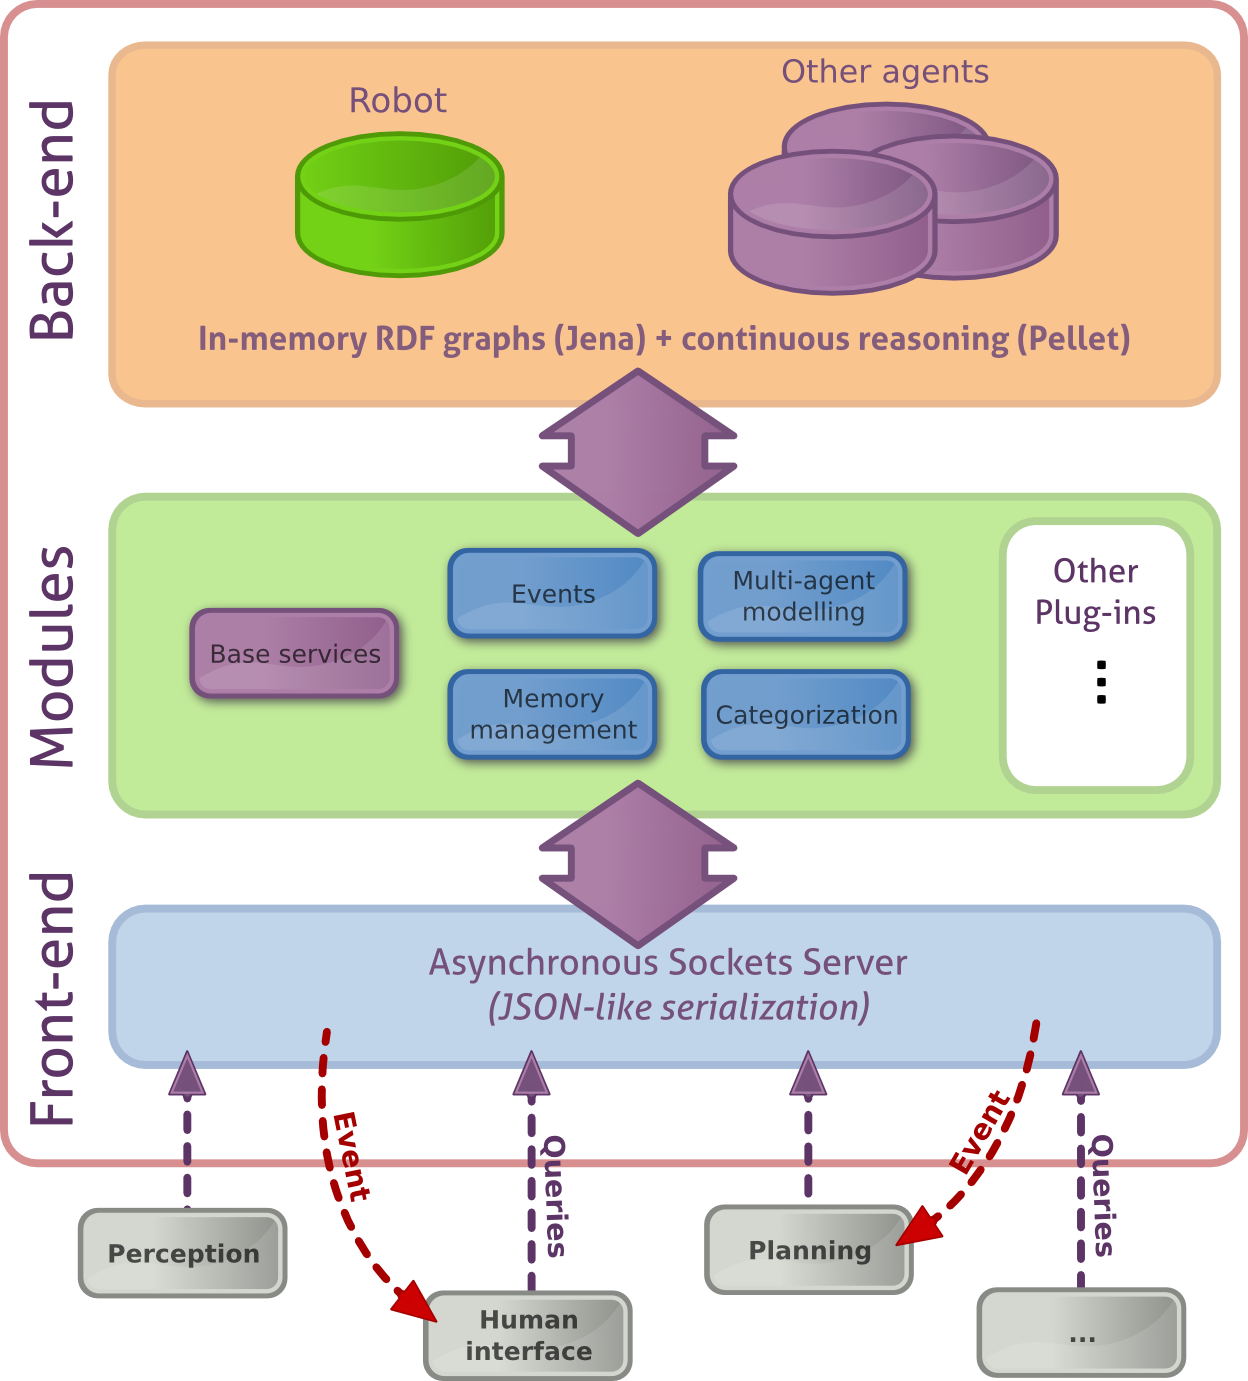
\includegraphics[width=0.8\linewidth]{images/oro_architecture.png}
  \caption{Overview of the ORO architecture.}
  \label{fig|oro-overview}
\end{figure}

\subsection{The OpenRobots Common-Sense Ontology}
\label{ontology}

The first requirement identified in section~\ref{knowledge_representation}
refers to the modeling of a cultural background, a common-sense knowledge
assumed to be shared by all agents.

The ORO server can be loaded with an initial set of statements which we call
the \emph{OpenRobots Common Sense Ontology}. It defines a small set of concepts
(and implicitly, a vocabulary) that can be used by all the modules of the robot
to unambiguously add or query facts. Moreover, the same ontology declares rules
and logical properties that are later on used for inference.

The \emph{OpenRobots Common Sense Ontology} defines a small set of classes (56
are currently defined) and predicates (60 are currently defined) focused on
concepts useful for human-robot interaction. It includes both very broad
categories like \concept{SpatialThing}, \concept{Event} or \concept{Action},
and much more concrete concepts as \concept{Table}, \concept{Book} or colors.
Available predicates allow us to describe the state of the agents and the world
with relations like \concept{isOn}, \concept{sees},
\concept{currentlyPerforms}, etc.

Several significant projects are trying to provide such a machine-processable
repository of common sense facts produced by humans (the \textsc{OpenMind}
project\footnote{\url{http://www.openmind.org/}}, for instance). These
knowledge bases are valuable but remain difficult to use in a pervasive way
because of both their incompleteness and the lack of good connections with
underlying, unambiguous concepts.
%\cite{Singh2002}

Our common sense ontology is closely aligned with the open-source
OpenCyc\footnote{\url{http://www.opencyc.org}} upper ontology.
OpenCyc defines a large taxonomy of concepts and semantic
relationships between concepts that are used in several other projects
(\textsc{WordNet, DBpedia}). This potentially eases the exchange and addition
of knowledge from these other sources. Moreover, it also enables knowledge
exchange with other robots (for instance, the works previously mentioned by
Daoutis and Tenorth rely on the same Cyc concepts\fixme{Give
examples}).

Figure~\ref{fig|oro-view} shows a snapshot of the knowledge model during an
experiment. Both concepts from the common sense ontology and
experiment-specific instances are visible.

\subsection{Reasoning and dynamic knowledge structuring}

As previously mentioned, ontologies in ORO are written in OWL, a language
based on Description Logics (a decidable subset of first-order logic). The
Pellet reasoner supports most of the OWL constructs and allows several type of
reasoning:

\begin{itemize}
	\item inheritance
	\item property axioms
		\begin{itemize}
		\item entailments based on predicates' domain and range,
		\item cardinality constraints (including \concept{allValue}, 
		\concept{someValue}, \concept{hasValue}),
		\item property characteristics (symmetry, transitivity)
		\end{itemize}
	\item class restrictions like: \par \footnotesize \concept{Bottle} $\equiv$
		\concept{Artifact} {\bf that} (\concept{hasShape} {\bf value}
		\concept{cylinderShape})\footnote{This example uses the \emph{Manchester
		syntax}, \url{http://www.w3.org/TR/owl2-manchester-syntax/}} \normalsize
	\item set operations like: \par \footnotesize \concept{Color} $\equiv$ {\bf unionOf}(\concept{blue},
		\concept{green}, \concept{orange}, \concept{black}...) \normalsize
	\item generic SWRL ({\em Semantic Web Rule Language}) rules like: \par
		\footnotesize \concept{looksAt(?agt, ?obj)} $\land$
		\concept{pointsAt(?agt,?obj)} $\Rightarrow$ \concept{focusesOn(?agt, ?obj)}
		\normalsize 
	\end{itemize}

We provide in ORO accessors to query, add or remove all these properties and
restrictions (except the SWRL rules) at run-time. This allows
knowledge introspection and enables the robot to alter its own knowledge
structures (the so-called \emph{T-Box} model) during its life-time by adding
new constraints and properties to classes and predicates.

The \emph{Naming} experiment (section~\ref{naming}) gives a simple example of
such knowledge restructuring.

\subsection{ORO features}
\label{features}

Besides storing and reasoning about knowledge, we have developed in ORO several
features to manage knowledge at higher level: 
%independent cognitive models for
%each agent the robot interacts with, categorization capabilities, different
%profiles of memory and events registration.

\subsubsection{Base functionalities}
\label{base}

ORO offers an extended set of methods to process facts at the triples level,
including:
\begin{itemize}
	\item statement (\ie RDF triples) insertion, removal, update,

	\item pattern-based statements removal,

	\item pattern-based queries (for instance, \stmt{ * isOn
	table}, which means ``return me all objects on table'') and filters (for
	instance, \concept{weight < 150.0}),

	\item consistency check, insertion of statements with consistency
	constraint (only if the new fact does not lead to inconsistencies),
	
	\item fast concept lookup, with possible multi-lingual support (through the
	\concept{@lang} XML annotation, labels of concept can be translated, and
	specific translations can be queried for),

	\item standard SPARQL queries.

\end{itemize}

While these basic functionalities enable the incremental construction (and
exploitation) of a consistent knowledge model, the \emph{Common Sense Ontology}
helps build assertions that are related to previous one by offering
a predefined vocabulary.

\subsubsection{Representation of alternative cognitive models}
\label{alterite}

As pictured in Figure~\ref{fig|oro-overview}, ORO stores independent cognitive
models for each agent it interacts with. When ORO actually identifies a new
agent (or infers that some instance is an agent), it automatically creates a
new, separate, in-memory OWL model for that agent. Thus, different robot
components, like supervision or situation assessment, may then store the
agents' beliefs in separate models. All knowledge processing functions in the
robot's primary model are equally available in every agent's model, which
allows us to store and reason on different (and possibly globally inconsistent)
models of the world.

This feature actually allows us to consider the robot to be endowed with a
\emph{theory of mind}~\cite{Scassellati2002}: the robot can explicitly model
the belief state of its interactors, opening new possibilities for the control
architecture. In section~\ref{dialog} we present how we use this feature to
make sense of user sentences from his/her point of view. Moreover,
these multiple models can be viewed as different interpretive scopes,
allowing the robot to interpret the same reality from different points of view.

\subsubsection{Categorization}
\label{categorization}

We have implemented several algorithms (common ancestors, computation of the
best discriminant, see~\cite{Ros2010b}) to help the robot cluster a set of
concepts based on their symbolic similarities (common properties, common
ancestors). One particular application of these functions is discrimination.
While interacting with a user, the robot quite often needs to clarify an
ambiguity produced by its human partner. For instance, a user may refer to a
``bottle'' where two bottles are currently visible. Discrimination routines
can identify possible (symbolic) differences (\eg the color or the size of the
bottles) that permit the robot to ask an accurate question to the user in order
to solve the ambiguity. This discrimination can occur from the robot's
perspective or from a specific agent's perspective. Usage of these
categorization abilities are illustrated in the \emph{Spy Game}
(section~\ref{spygame}).

\subsubsection{Memory profiles}
\label{memory}

We have designed a simplified bio-inspired memory model that allows us to store
statements in different \emph{memory profiles}. These include \emph{short term
memory} and \emph{long term memory}. Each profile is characterized with a
lifetime, which is assigned to the stored facts. When the lifetime of a fact
expires, ORO automatically removes it.

\subsubsection{The events framework} 
\label{events} 

Lastly, ORO allows external modules to be triggered when specific events occur,
 for instance, when a logical sentence becomes true or false, or if a new
instance of a certain class is added. One immediate application is reactive
supervision: a component could for instance subscribe to events of kind
\setstmt{?agent isVisible true, ?agent type Human}. As soon as the perception
layer detects a human in the robot's field of view and accordingly updates the
knowledge base, the supervision component would be triggered back. The event
framework also takes advantage of the inference capabilities of ORO. Thus an
event can be indirectly triggered if its triggering conditions can be inferred
to be true.

Next sections describe how symbolic knowledge is actually produced and added to
ORO.

%%%%%%%%%%%%%%%%%%%%%%%%%%%%%%%%%%%%%%
\section{Geometric reasoner for situation assessment} 

Anchoring perceptions in a symbolic model requires perception abilities
and their symbolic assessments. In this section we present
SPARK (\emph{SPAtial Reasoning \& Knowledge}, \cite{Sisbot2011}), a situation assessment reasoner
that generates relevant symbolic information from the geometry of the
environment with respect to relations between objects, robots and humans.
Moreover, the notion of \emph{Perspective
Taking}~\cite{Flavell1992,Tversky1999} is employed at the heart of the
reasoner to provide the robot with the ability to put itself at the human's
place and to reason about the world from different perspectives.

As mentioned in the introduction, this paper does not focus on the sensor-level
perception. We rather assume that the perception of the humans and the objects
is provided as a list of unique identifiers with associated 3D meshes and 6DOF
poses.

\subsection{Capabilities}

There are a number of common properties for a robot and a human related to
their capabilities in a given situation: they can both reach, grasp, look at,
point at, etc. In our context, we group robots and humans into a single category.
Thus, we define agents as entities that can act in the environment and
manipulate it. In this work we focus on the following capabilities from each
agent's perspective\footnote{Note that each of the capabilities described are
computed from each agent point of view, and therefore, also stored in different
models in ORO for further use at the decisional level.}:

\begin{itemize}

\item \emph{Sees}: An important ability to know about an agent is to predict
``what it can see'', \ie what is within its field of view (FOV). A robot being
able to compute this information can then act accordingly. A typical example
would be a clarification scenario where the human is searching for an object
and the robot is able to infer that it is looking for the one that is not
visible (otherwise the user would not be searching for it).

In figure~\ref{fig::vis} the field of view of a person is illustrated with a
grey cone (broader one). While he is able to see the two small boxes on the
table in front of the him, the big box on his right is out of this FOV, and
therefore, he is not able to see it. 

\item \emph{Looks At}: this relation corresponds to what the agent is focused
on, \ie where its focus of attention is directed. This model is based on a
narrower field of view, the field of attention (FOA). Figure~\ref{fig::vis}
shows the field of attention of a person with a green cone (narrower one). In
this example only the grey box satisfies the \concept{looksAt} relation.

\begin{figure}[!t] \centering
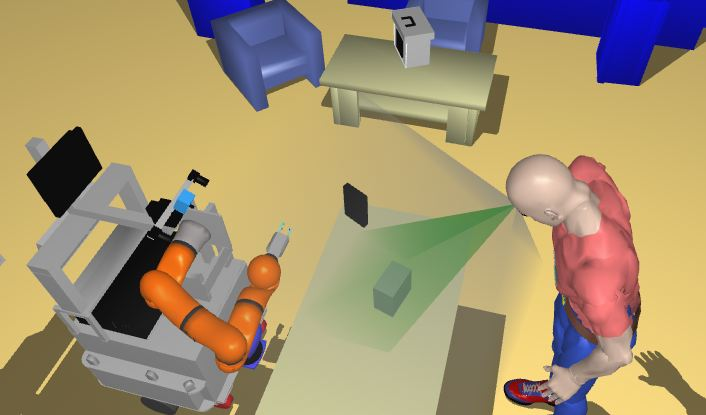
\includegraphics[width=\columnwidth]{images/looks.jpg} \caption{Representation
of the field of view (FOV) and the field of attention (FOA) of the human.}
\label{fig::vis} \end{figure}

\item \emph{Points At}: verifies whether an object is pointed at by an agent. This
relation is particularly useful during interaction when one of the agents is
referring to an object saying ``this" or ``that" while pointing at it. 
 
If a big object occludes a smaller one, and an agent is pointing at them, the
outcome of the evaluation will result only in one relation, \ie \stmt{agent\_01
pointsAt object\_01} since the small one is not visible to the agent.  On the
contrary, if the small object is in front of the big one, then both objects
will satisfy the relation, which may generate an ambiguity (which object the
agent refers to?) that should be solved through higher level reasoning (\eg
context analysis or clarification through verbal interaction as shown later
on).

\item \emph{Reachable}: it allows the robot to estimate the agent's capability
to reach an object, which is fundamental for task planning. For example, if the
user asks the robot to give her an object, the robot must compute a transfer
point where the user is able to get the object afterward. 

Figure~\ref{fig::reach} shows different reachability postures for each object
on the table. In the example, the bottle and the box are both reachable by the
human, but the teddy bear is too far. Instead, from the robot's perspective,
the teddy bear is reachable, while the bottle is not.

\begin{figure}[!t] 
	\centering
	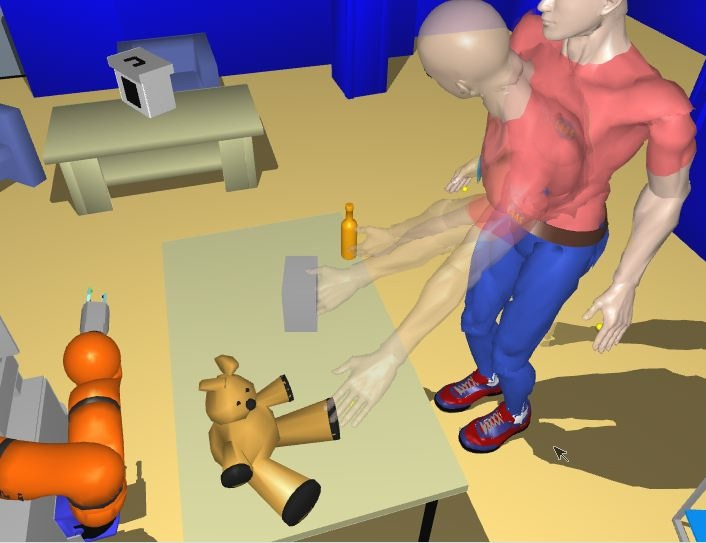
\includegraphics[width=\columnwidth]{images/reach.jpg} 
	\caption{Different reaching postures for the human: the bottle and the 
	box are reachable, while the teddy bear is not.} 
	\label{fig::reach} 
\end{figure} 

\end{itemize}

While the first three relations (\concept{sees}, \concept{looksAt} and
\concept{pointsAt}) are computed through a model based approach, the latter one
is based on the Generalized Inverse Kinematics with pseudo inverse
method~\cite{Nakamura90,Baerlocher04} to find a collision free posture for the
agent where its end-effector is at the center of the object within a given
tolerance. The details of these computations are out of the scope of this
article.

\subsection{Locations}

One way of referring to object's
positions is based on a human's symbolic descriptors, instead of using their precise
position. In fact, in many cases, this information is the most precise information available
 since we do not store the numeric coordinates of objects. The
following relations are computed with respect to the position of the agents and
the objects.

\begin{itemize} 

\item \emph{Location according to an agent}: The predicate
\concept{isLocatedAt} represents spatial locations between agents and objects.
For example we say ``it is on my right, on your left, ...'' These type of direction commands are studied
in the literature in the context of language grounding (\eg \cite{OKeefe1999,Matuszek10}). We compute these
spatial locations by dividing the space around the referent (an agent) into $n$
regions based on arbitrary angle values relative to the referent orientation.
For example, for $n = 4$ we would have the space divided into \emph{front,
left, right} and \emph{back}. Additionally, two proximity values, \emph{near}
and \emph{far}, may also be considered. The number of regions and proximity
values can be chosen depending on the context where the interaction takes
place.

\item \emph{Location according to an object}: We can also refer to object
locations with respect to other objects in the environment, such as \emph{above,
next to, in}, etc. These types of relations are widely studied in language
grounding (\eg \cite{Regier01} presented different models to define the
\emph{above} relation; \cite{Kelleher09} presented two computational models of topological and projective spatial prepositions; \cite{Blisard05} employed contour points of segmented objects to determine \emph{front, behind, left,right} relations). In this work we use similar models based on the
bounding boxes and center of mass of the objects to define three main relations
(Figure~\ref{fig::sprelation}): 

\begin{itemize}
	\item \concept{isOn}: computes if an object $O_1$ is on another object $O_2$ by
	evaluating the center of mass of $O_1$ according to the bounding box of $O_2$.

	\item \concept{isIn}: evaluates if an object $O_1$ is inside another object
	$O_2$ based on their bounding boxes $BB_{O_1}$ and $BB_{O_2}$.

	\item \concept{isNextTo}: indicates whether an object $O_1$ is next to another
	object $O_2$. We cannot use a simple distance threshold to determine if two
	objects are next to each other since the relation is highly dependent on the
	dimensions of the objects. For instance, the maximum distance between large
	objects (\eg two houses) to consider them as being next to each other is much
	larger than the maximum distance we would consider for two small objects (\eg
	two bottles). Thus, the relation between the dimensions and the distances of
	the objects are taken into account.  

\begin{figure} 
	\centering
	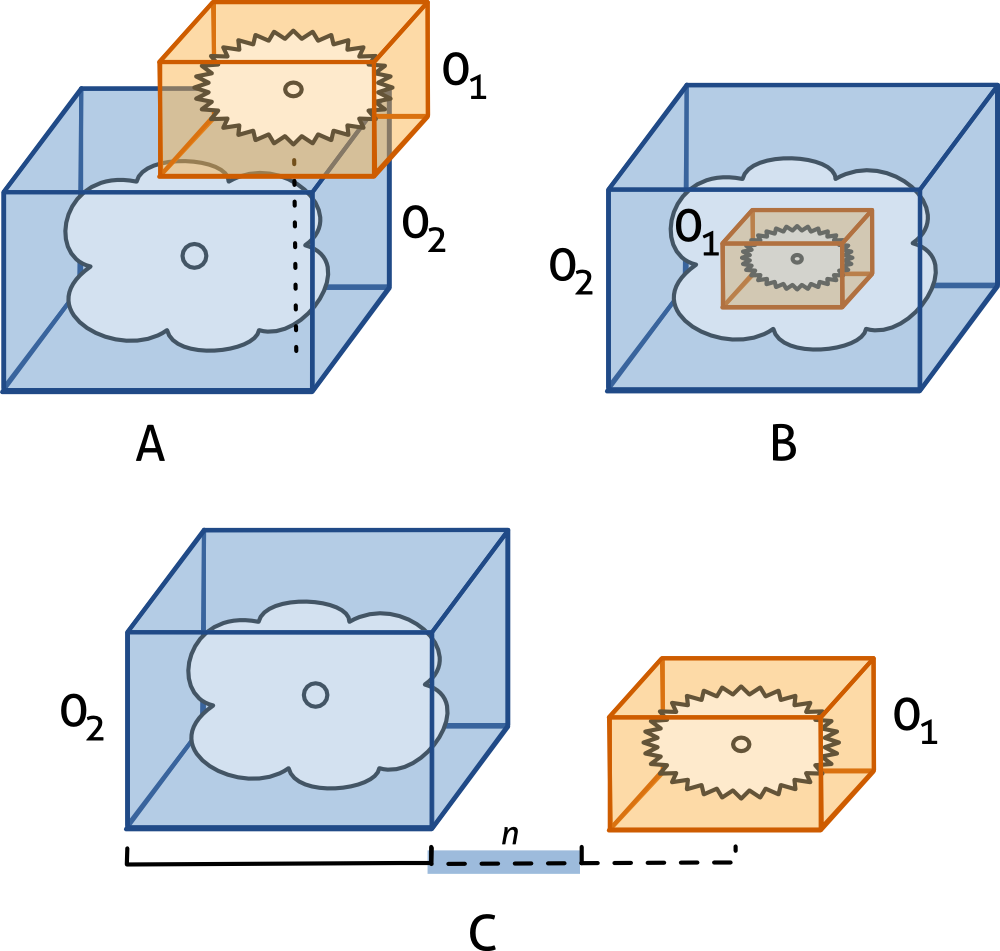
\includegraphics[width=0.8\columnwidth]{images/spatial_relation.png}
	\caption{Spatial relations between two objects: A) \concept{isOn} relation, 
	B) \concept{isIn} relation, and C) \concept{isNextTo} relation.} 
	\label{fig::sprelation} 
\end{figure}

\end{itemize} 
\end{itemize}

To ensure the different agent's models are up-to-date, all these properties are
always computed on-line, each time the current state of the world changes.

SPARK can be compared to the \emph{Grounded Situation Model} (GSM) introduced
by Mavridis and Roy~\cite{Mavridis2005} in the sense that they both provide an
amodal physical representation of the world used as a mediator between the
sensor space and symbolic models. They have however a different set of
features: while GSM enables representation of time and imaginary objects (whose
existence is hinted by verbal assertions from a human, also called
\emph{presupposition accomodation}), SPARK offers a richer 3D model that
enables the computation of several spatial relationships between
objects and an effective implementation of perspective taking capabilities.

%%%%%%%%%%%%%%%%%%%%%%%%%%%%%%%%%%%%%%
\section{The natural language grounding process}
\label{dialog}

Verbal interaction with human presents two categories of challenges: syntactic
ones, and semantic ones. The robot must be able to process and analyze the
structure of human utterances, \ie natural language sentences, and then make
sense of them. As stated in the introduction, we process three categories of
sentences: \emph{statements}, \emph{desires} and \emph{questions} that can be
answered from the declarative knowledge present in the robot knowledge base (a
choice similar to the \emph{Behaviour Cycle} in the GLAIR
architecture~\cite{Shapiro2009}). In our work, the grounding process of the
human discourse consists in extracting either the \emph{informational} content
of the sentence to produce statements or its \emph{intentional} content (\ie
performative value) to collect orders and questions. We do not claim any
contribution to the field of computational linguists (see \cite{Kruijff2010}
for a survey of formal approaches to natural language processing in the
robotics field). Our main contribution here is the grounding (we call it
\emph{resolution}) of concepts involved in the human discourse through the
robot's own knowledge.

We have developed a dedicated module called {\sc Dialogs} that processes human
input in natural language, grounds the concepts in the robot's knowledge and
eventually translates the discourse in a set of queries or declarative OWL/RDF
statements.

\begin{figure}[!ht]
\centering
  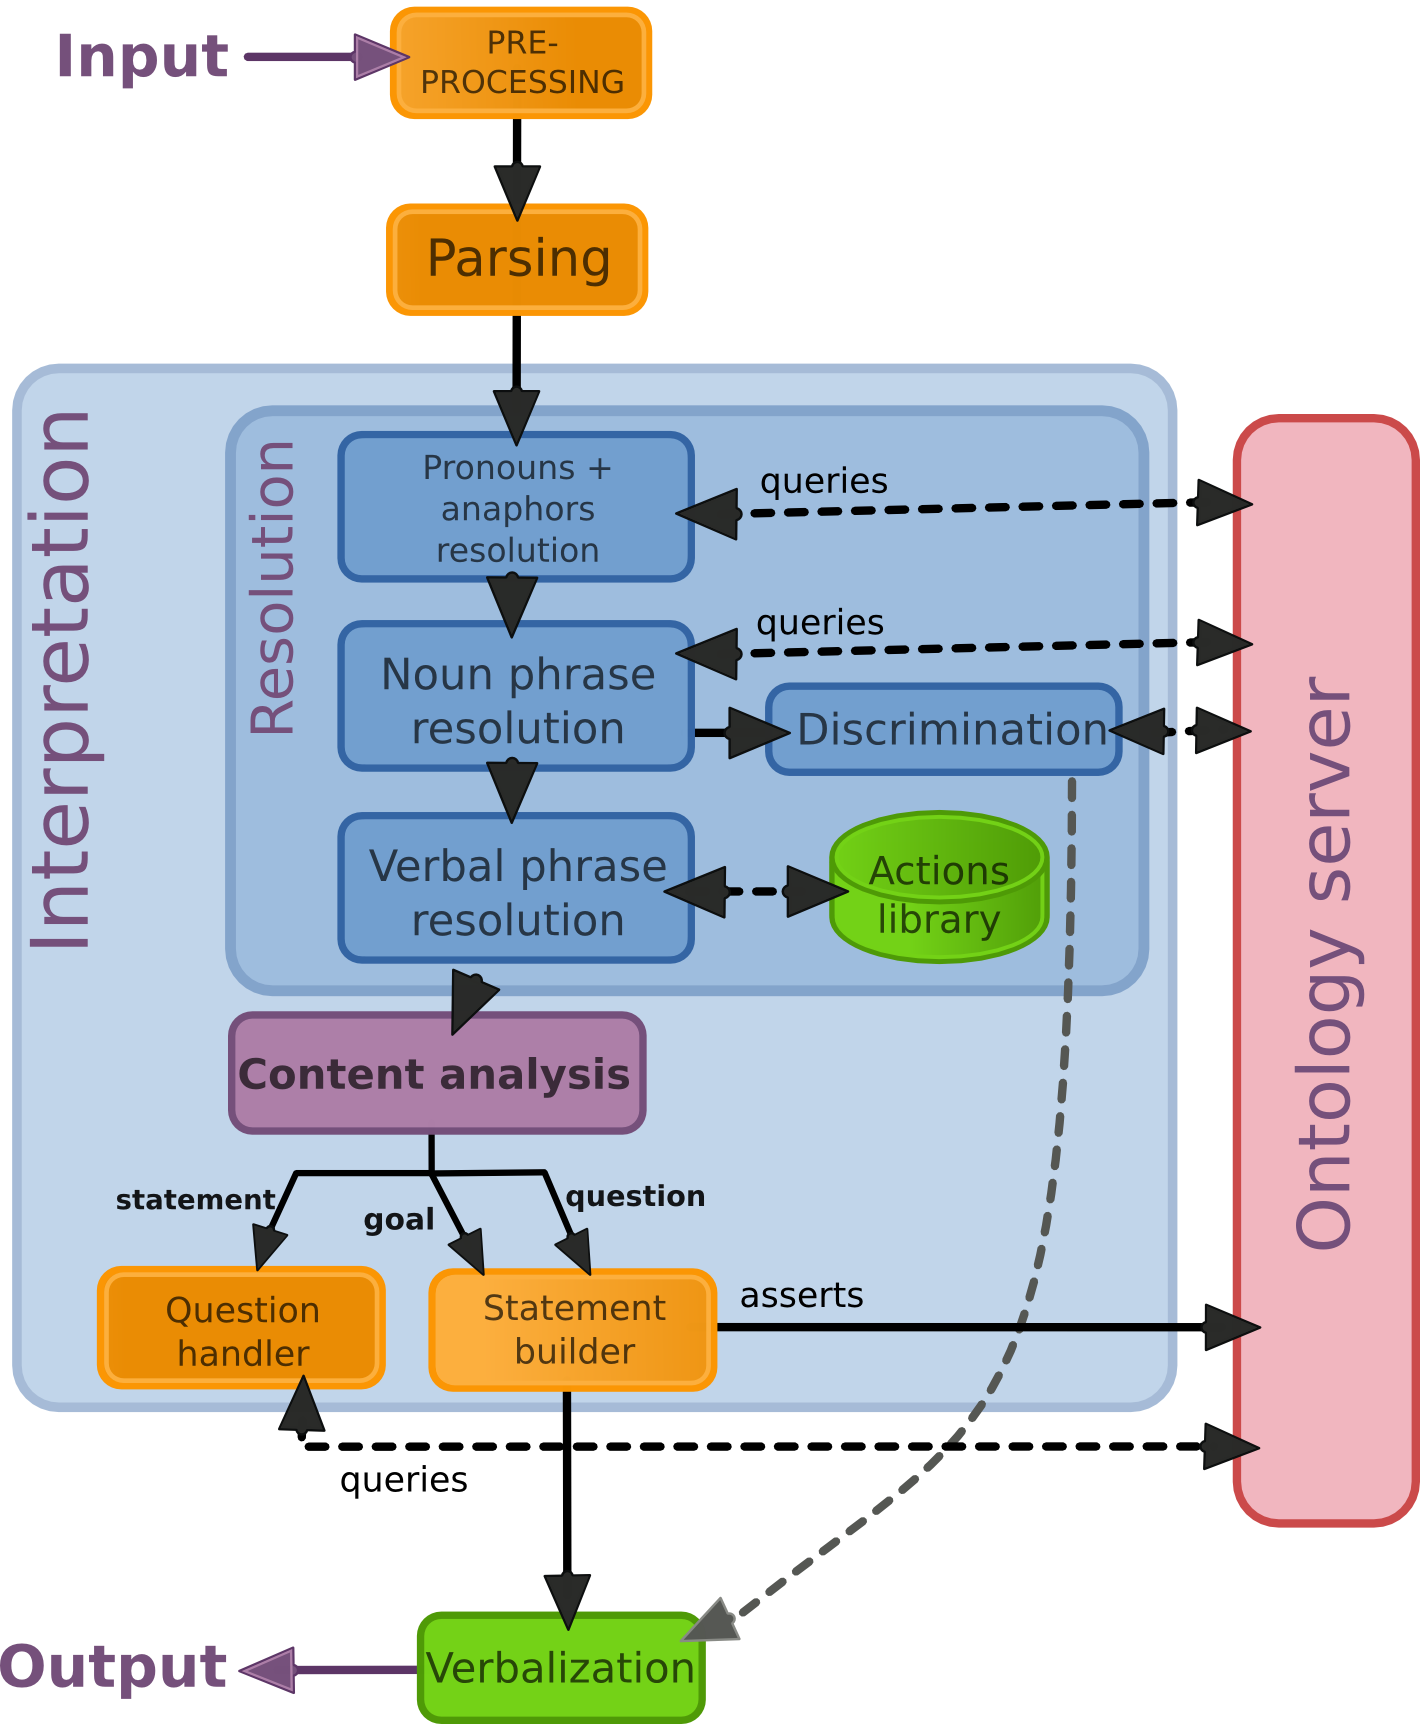
\includegraphics[width=0.9\linewidth]{images/dialog_module_simple.png}
  \caption{The {\sc Dialogs} module has three main steps: the parsing,
  the interpretation and the verbalization. The interpretation module is
  responsible for both the \emph{resolution} and the semantic content
  \emph{analysis and translation}.} 
  \label{fig|dialog}
\end{figure}

Figure~\ref{fig|dialog} shows the {\sc Dialogs} module architecture. The user's
input is first pre-processed. For instance, \emph{I'm} constructs are expanded
into \emph{I am} and then parsed. The parser is a custom-made, rule-based (\ie
grammar-free) tool that extracts the grammatical structure from the user's
sentence. Figure~\ref{dialog|parser_output} shows the raw output of the parser for a
moderately complex sentence.

\begin{figure}[!ht]
\begin{center}
\scriptsize
\begin{alltt}
>> IMPERATIVE
VP: \textbf{remember} (present simple)
    SUBSENTENCE (aim: that)
      NP: \textbf{I}
      VP: \textbf{want} (present simple)
        direct objects: 
          NP: \textbf{you}
        secondary VP: \textbf{give} ()
              direct objects:
                NP: my \emph{nice blue} \textbf{bottle}
              indirect objects:
                NP: \textbf{me}
\end{alltt}
\end{center}
\caption{Raw output of the {\sc Dialogs} parser after processing the
sentence: ``remember that I want you to give me my nice blue bottle.'' 
Nominal groups are not grounded yet.} 
\label{dialog|parser_output}
\end{figure}

The output of the parser is then sent to the \emph{interpretation} module, the
core of the component.  Interpretation consists in three distinct operations:
the sentence \emph{resolution} (concepts grounding), the \emph{content
analysis} (what is the intent of the utterance: information, question or
desire) and the \emph{statement building} (translation into RDF statements).

The sentence resolution has three steps: {\it(1)} pronouns and anaphora are
replaced by the correct speaker ID and the ID of the last object spoken about
(extracted from the dialogue history) respectively, {\it(2)} nominal groups are
disambiguated and grounded (noun phrase resolution, \cf below), and {\it(3)}
verbal groups are resolved and their associated \emph{thematic roles} are
retrieved (verbal phrase resolution).

\small
\begin{pseudocode}[ruled]{Resolution}{sentence, currentSpeaker}
\label{algo|Resolution}

\mathcal{G} \GETS \CALL{ParseNominalGroups}{sentence} \\

\FOREACH g \in \mathcal{G} \DO 
\BEGIN
   \mathcal{D} \GETS \CALL{GenerateDescription}{g} \STMTNUM{5.1em}{res.desc}\\
   candidates \GETS \CALL{Ontology.Find}{\mathcal{D}} \STMTNUM{4em}{res.onto}\\
   
   \IF \left|{candidates}\right| = 0 \THEN
    \BEGIN
      \OUTPUT{\mbox{Couldn't resolve the group!}} \\
      \EXIT \\
    \END
   \ELSEIF \left|{candidates}\right| = 1 \THEN
      id \GETS candidates[0] \STMTNUM{8em}{res.easy}\\

   \ELSE
      \BEGIN
	\IF \CALL{Ontology.CheckEquivalent}{candidates} \THEN
	  id \GETS candidates[0] \\
	\ELSE
	  id \GETS \CALL{Discrimination}{candidates} \\ %\STMTNUM{0em}{st.discrimination}\\
      \END \\
   \CALL{Replace}{g, id, sentence}
\END
\end{pseudocode}
\normalsize

As represented in Figure~\ref{fig|dialog}, interpretation tightly relies on the
communication with the knowledge base. All the concepts the robot manipulates
are stored in the \textit{ontology server} and retrieved through logical
queries, except for the verbs that are currently stored in a dedicated library
(the \emph{action library} in the diagram).

%%%%%%%%%%%%%%%%%%%%%%%%%%%%%%%%%%%%%
\section{Technical analysis}
\label{examples}


In order to better understand the overall process we next describe the
different steps of the approach based on three examples. In these examples, we
assume that some initial facts are present in the knowledge base, both in the
robot's own model and in the human's model.  Since the robot tries to ground a
human utterance, all queries are sent to the human model in order to interpret
it from the human perspective. 

\subsection{Informational content extraction}

Figure~\ref{dialog|ex1} shows a first example of human discourse grounding and
the extraction of informational content. We assume that the robot knowledge
base only contains two initial statements in the human model. The user
asserts a new one: ``The yellow banana is big!''. 

\begin{figure}
    \centering
	\begin{tabular}{p{7cm}}
	\emph{Initial knowledge model of} \texttt{human\_01}\\
	\hline
    	\hspace{0.3cm}\stmt{banana\_01 type Banana} \\
    	\hspace{0.3cm}\stmt{banana\_01 hasColor yellow}\\
	
	\vspace{0.5em}
	\emph{Human input}\\
	\hline
	\hspace{0.3cm}``The yellow banana is big!'' \\

	\vspace{0.5em}
	\emph{Generated partial statements}\\
	\hline
	\hspace{0.3cm}\stmt{?obj type Banana} \\
    	\hspace{0.3cm}\stmt{?obj hasColor yellow} \\
    	\hspace{0.7cm}$\Rightarrow$ \concept{?obj = banana\_01}\\

	\vspace{0.5em}
	\emph{Newly created statements}\\
	\hline
	\hspace{0.3cm}\stmt{banana\_01 hasSize big} \\
	\end{tabular}
\caption{First example of natural language grounding: the nominal group ``the
yellow banana'' is matched with the individual \concept{banana\_01}.
``$\Rightarrow$'' represents the output of the ontology server.}
\label{dialog|ex1}
\end{figure}

We first want to match the nominal group \emph{The yellow banana} to an already
known concept, and second to translate the property \emph{is big} into a
predicate (\emph{hasSize}) to state its semantics. The general resolution
algorithm of nominal groups is described in algorithm~\ref{algo|Resolution}.

To resolve the nominal group \emph{The yellow banana} a set of partial
statements that describe the concept is generated based on the grammatical
parsing of the sentence (algorithm~\ref{algo|Resolution},
\emph{(\ref{res.desc})}). In the example, a banana (\stmt{?obj type Banana})
that is yellow (\stmt{?obj hasColor yellow})\footnote{Predicates like
\concept{hasColor} or \concept{hasSize} that bind \concept{banana\_01} to
adjectives are extracted from a predefined database of $[Predicate \rightarrow
AdjectiveCategory]$, and falls back on the generic \concept{hasFeature}
predicate if the adjective is not known.}.  Based on these partial statements a
query is sent to the ontology server to retrieve possible instances that match
the description (algorithm~\ref{algo|Resolution}, \emph{(\ref{res.onto})}).

In this first simple case, the concept \concept{banana\_01} is unambiguously
matched (since there is only one possible banana) and returned. Finally, we can now add
the new information provided by the human, \ie the new statement
\stmt{banana\_01 hasSize big}, to the human model in the ontology
server.

% The translation of \emph{yellow} to \stmt{hasColor yellow} is not obvious: in
% the general case, we associate a adjective to the noun it characterizes with
% the \concept{hasFeature} predicate (for instance, \emph{The sight is beautiful}
% would translate to \stmt{sight hasFeature beautiful}). But we can also manually
% set the predicate associated to a category of adjectives: It is what has been
% done for the main colours. Another example is the size: for known size
% adjectives (big, small, etc.), the \concept{hasSize} predicate is being used.

\subsection{Intentional content through verb resolution}
The sentence in the first example is built with the state verb \emph{be} at
indicative. Let us examine a different example with an action verb at
imperative mode (an order): ``Give me the banana". The process is
described in Figure~\ref{dialog|ex2}.

\begin{figure}
    \centering
	\begin{tabular}{p{7cm}}
	\emph{Initial knowledge model of} \texttt{human\_01}\\
	\hline
    	\hspace{0.3cm}\stmt{banana\_01 type Banana} \\
    	\hspace{0.3cm}\stmt{banana\_01 hasColor yellow}\\
	\end{tabular} \\

	\vspace{0.5em}

	\begin{tabular}{p{7cm}}
	\emph{Human input}\\
	\hline
    	\hspace{0.3cm}``Give me the banana.'' \\
	\end{tabular} \\

	\vspace{0.5em}

	\begin{tabular}{p{7cm}}
	\emph{Generated partial statements}\\
	\hline
    	\hspace{0.3cm}\stmt{?obj type Banana} \\
	\hspace{0.7cm}$\Rightarrow$ \concept{?obj = banana\_01}\\

	\end{tabular} \\

	\vspace{0.5em}

	\begin{tabular}{p{7cm}}
	\emph{Newly created statements}\\
	\hline
    	\hspace{0.3cm}\stmt{human\_01 desires situation\_a3f74} \\
    	\hspace{0.3cm}\stmt{situation\_a3f74 type Give} \\
    	\hspace{0.3cm}\stmt{situation\_a3f74 performedBy myself} \\
    	\hspace{0.3cm}\stmt{situation\_a3f74 actsOnObject banana\_01} \\
    	\hspace{0.3cm}\stmt{situation\_a3f74 receivedBy human\_01} \\
	\end{tabular}

\caption{Second example: processing an order.}
\label{dialog|ex2}
\end{figure}

\label{processing_of_actions}

In order to capture the intentional content of a sentence (for example, an
order) we need to retain the semantics of the verb and its complements.
\emph{Thematic roles} allow for semantically linking a verb to its complements.  
There is no general agreement amongst linguists on a comprehensive list of 
thematic roles. The amount and the granularity of roles varies a lot in 
the literature~\cite{Gutierrez2001}. We thus use a small set of them, which matches
the relations the robot can actually achieve (we discuss
possible extensions in the conclusion). For instance, in the second example,
the verb \emph{give} has three thematic roles: \concept{performedBy},
\concept{actsOnObject} and \concept{receivedBy}.

The list of actions the robot can plan for (currently \emph{take},
\emph{place}, \emph{give}, \emph{show}, \emph{hide} and \emph{move}) along with
possible synonyms (for example, \emph{to pick} is set as a synonym of \emph{to
take}) and their associated thematic roles are stored in a predefined library
of actions. For each action we identify and store: the role of the subject in
the sentence (always \concept{performedBy}); the role of the direct object
(for instance, \concept{actsOnObject}); and the role of each of the indirect
objects with their optional prepositions (for instance,
\concept{receivedBy})\footnote{Note that in example 2, ``give me the banana'',
the pronoun ``me'' appears before ``banana'', while it is an indirect
complement --- ``give it {\bf to me}''. The parser correctly handles these
cases.}. Moreover, through the ontology we check that each holder of a
role is semantically consistent. For instance, the action \emph{Give} must have a
manipulable physical item (\concept{Artifact}) as direct object. Thus, if the
concept the robot finds for the thematic role \concept{actsOnObject} can not be
inferred to be an artifact, the robot goes back to the human saying it does not
understand.

This second example  also shows the pronouns reference resolution: ``me'' is
replaced by the id of the current speaker while ``you'' is replaced by
\concept{myself} (\concept{myself} always represents the robot itself). When
present, anaphoras (references to previous concepts like ``give me the banana, I
like {\bf it}.'') are also resolved in the same step.

Once the sentence is completely resolved and translated into a formal
representation (a human desire in this example\footnote{Orders are here
represented as human desires: the human desires a specific new situation.}), we
store it in the ontology server. The robot's decisional/executive layers can
then decide whether to execute the order or not. 

\subsection{Informational content extraction requiring clarification}
\begin{figure}
    \centering
	\begin{tabular}{p{7cm}}
	\emph{Initial knowledge model of} \texttt{human\_01}\\
	\hline
     	\hspace{0.3cm}\stmt{banana\_01 type Banana} \\
     	\hspace{0.3cm}\stmt{banana\_01 hasColor yellow} \\
     	\hspace{0.3cm}\stmt{banana\_02 type Banana} \\
     	\hspace{0.3cm}\stmt{banana\_02 hasColor green} \\
	\end{tabular} \\

	\vspace{0.5em}

	\begin{tabular}{p{7cm}}
	\emph{Human input}\\
	\hline
     	\hspace{0.3cm}``The banana is good.'' \\
	\end{tabular} \\

	\vspace{0.5em}

	\begin{tabular}{p{7cm}}
	\emph{Generated partial statements}\\
	\hline
     	\hspace{0.3cm}\stmt{?obj type Banana} \\
	\hspace{0.7cm} $\Rightarrow$ \concept{?obj = [banana\_01, banana\_02]}
	\end{tabular} \\

	\vspace{0.5em}

	\begin{tabular}{p{7cm}}
	\emph{Discrimination process}\\
	\hline
     	\hspace{0.3cm}\concept{discriminate([banana\_01, banana\_02])} \\
	\hspace{0.7cm} $\Rightarrow$ \concept{?hasColor = [yellow, green]}
	\end{tabular} \\

	\vspace{0.5em}

	\begin{tabular}{p{7cm}}
	\emph{Robot output speech}\\
	\hline
     	\hspace{0.3cm}``The yellow one or the green one?'' \\
	\end{tabular} \\

	\vspace{0.5em}

	\begin{tabular}{p{7cm}}
	\emph{Human answer}\\
	\hline
     	\hspace{0.3cm}``The green one.'' \\
	\end{tabular} \\
    
	\vspace{0.5em}

	\begin{tabular}{p{7cm}}
	\emph{Extended human input}\\
	\hline
     	\hspace{0.3cm}``The green banana is good.'' \\
	\end{tabular} \\
	
	\vspace{0.5em}

	\begin{tabular}{p{7cm}}
	\emph{Generated partial statements}\\
	\hline
     	\hspace{0.3cm}\stmt{?obj type Banana} \\
     	\hspace{0.3cm}\stmt{?obj hasColor green} \\
	\hspace{0.7cm} $\Rightarrow$ \concept{?obj = [banana\_02]}
	\end{tabular} \\
    
	\vspace{0.5em}
	\begin{tabular}{p{7cm}}
	\emph{Newly created statements}\\
	\hline
     	\hspace{0.3cm}\stmt{banana\_02 hasFeature good} \\
	\end{tabular}

\caption{Ambiguity resolution: in this example, ``banana'' can refer to the
yellow banana (\concept{banana\_01}) or the green one (\concept{banana\_02}).
Discrimination routines handle the disambiguation process.} \label{dialog|ex3}
\end{figure}

This last example (Figure~\ref{dialog|ex3}) shows the resolution of ambiguous
concepts. In this case the user refers to ``the banana'' while two instances of 
the \concept{Banana} class exist in the ontology. The robot needs to find out 
to which instance the user is actually referring to. To this end, 
disambiguation routines~\cite{Ros2010b} find differences between the instances 
(in the example, one banana is yellow while the other one is green) and build a 
sentence through the \emph{verbalization} module to ask the user a closed 
question that will help clarify the ambiguity: ``Is it yellow or green?'' The 
user's answer is parsed and merged with the previous sentence. The resulting, 
augmented, sentence (``The green banana is good") goes again through all 
the interpretation steps. This process is repeated until no ambiguities arise. 
In the example, the \concept{banana\_02} is finally returned.

%If no differences \fxfatal{should we say 'in the human model', even if 
%getDiscriminantForAgent currently doesn't work?} can be found, an open question 
%(``give me more information'') is send to the human.

Several other strategies are used in parallel to disambiguate concepts without
having to ask for more information to the human:

\begin{itemize}
	\item Which objects are currently visible to the human? If only one of
	them, then it is probably the one the user is talking about. 
	\item Did a previous interaction involved a specific object that would
	still be the subject of the current sentence?
	\item Is the user looking or pointing at a specific object?
\end{itemize}

%Two cases can alter the way the discrimination routines work:
%\begin{enumerate}
%    \item If a sentence starts with {\it Learn that...}, failures during 
%    discrimination are interpreted as new concepts, and instead of marking the 
%    nominal as not resolved, and new identifier is created and add to the knowledge base.
%    \item For questions like {\it Which color is the bottle?}, the discrimination 
%    algorithm can not use the feature {\it color} to identify to bottle. The 
%    resolution algorithm pass this kind of constraints as a parameter of the 
%    discrimination routines.
%\end{enumerate}

 
While no examples involving questions have been detailed, \emph{W-} questions
and \emph{yes/no} questions can be processed in a similar way by
\textsc{Dialogs}. For instance, a question like ``What is on the table?''
is grounded (to extract the relation \concept{isOn} and to find what \emph{table}
refers to) and transformed into the following kind of query: {\tt find ?var
[\stmt{?var isOn table1}]}.  Answers are converted back to a full sentence
by the \emph{verbalization} module, and uttered to the human.

%%%%%%%%%%%%%%%%%%%%%%%%%%%%%%%%%%%%%
\section{Experiments}

This section presents several experiments where the different features of our
approach are represented.

Experiments have been conducted on two different platforms: the
\emph{Rosie} manipulator from the Technical Universtiy of Munich, a dual-arm,
holonomic service robot, running the ROS\footnote{\emph{Robotic Operating
System}, \url{http://www.ros.org}} middleware, and the \emph{Jido} robot~\cite{Alami1998a} from
LAAS-CNRS, a similar, single-arm, service robot, running the LAAS's {\sc
Genom/pocolibs} stack.

\subsection{\emph{Naming} experiment}
\label{naming}

\begin{figure}
\centering
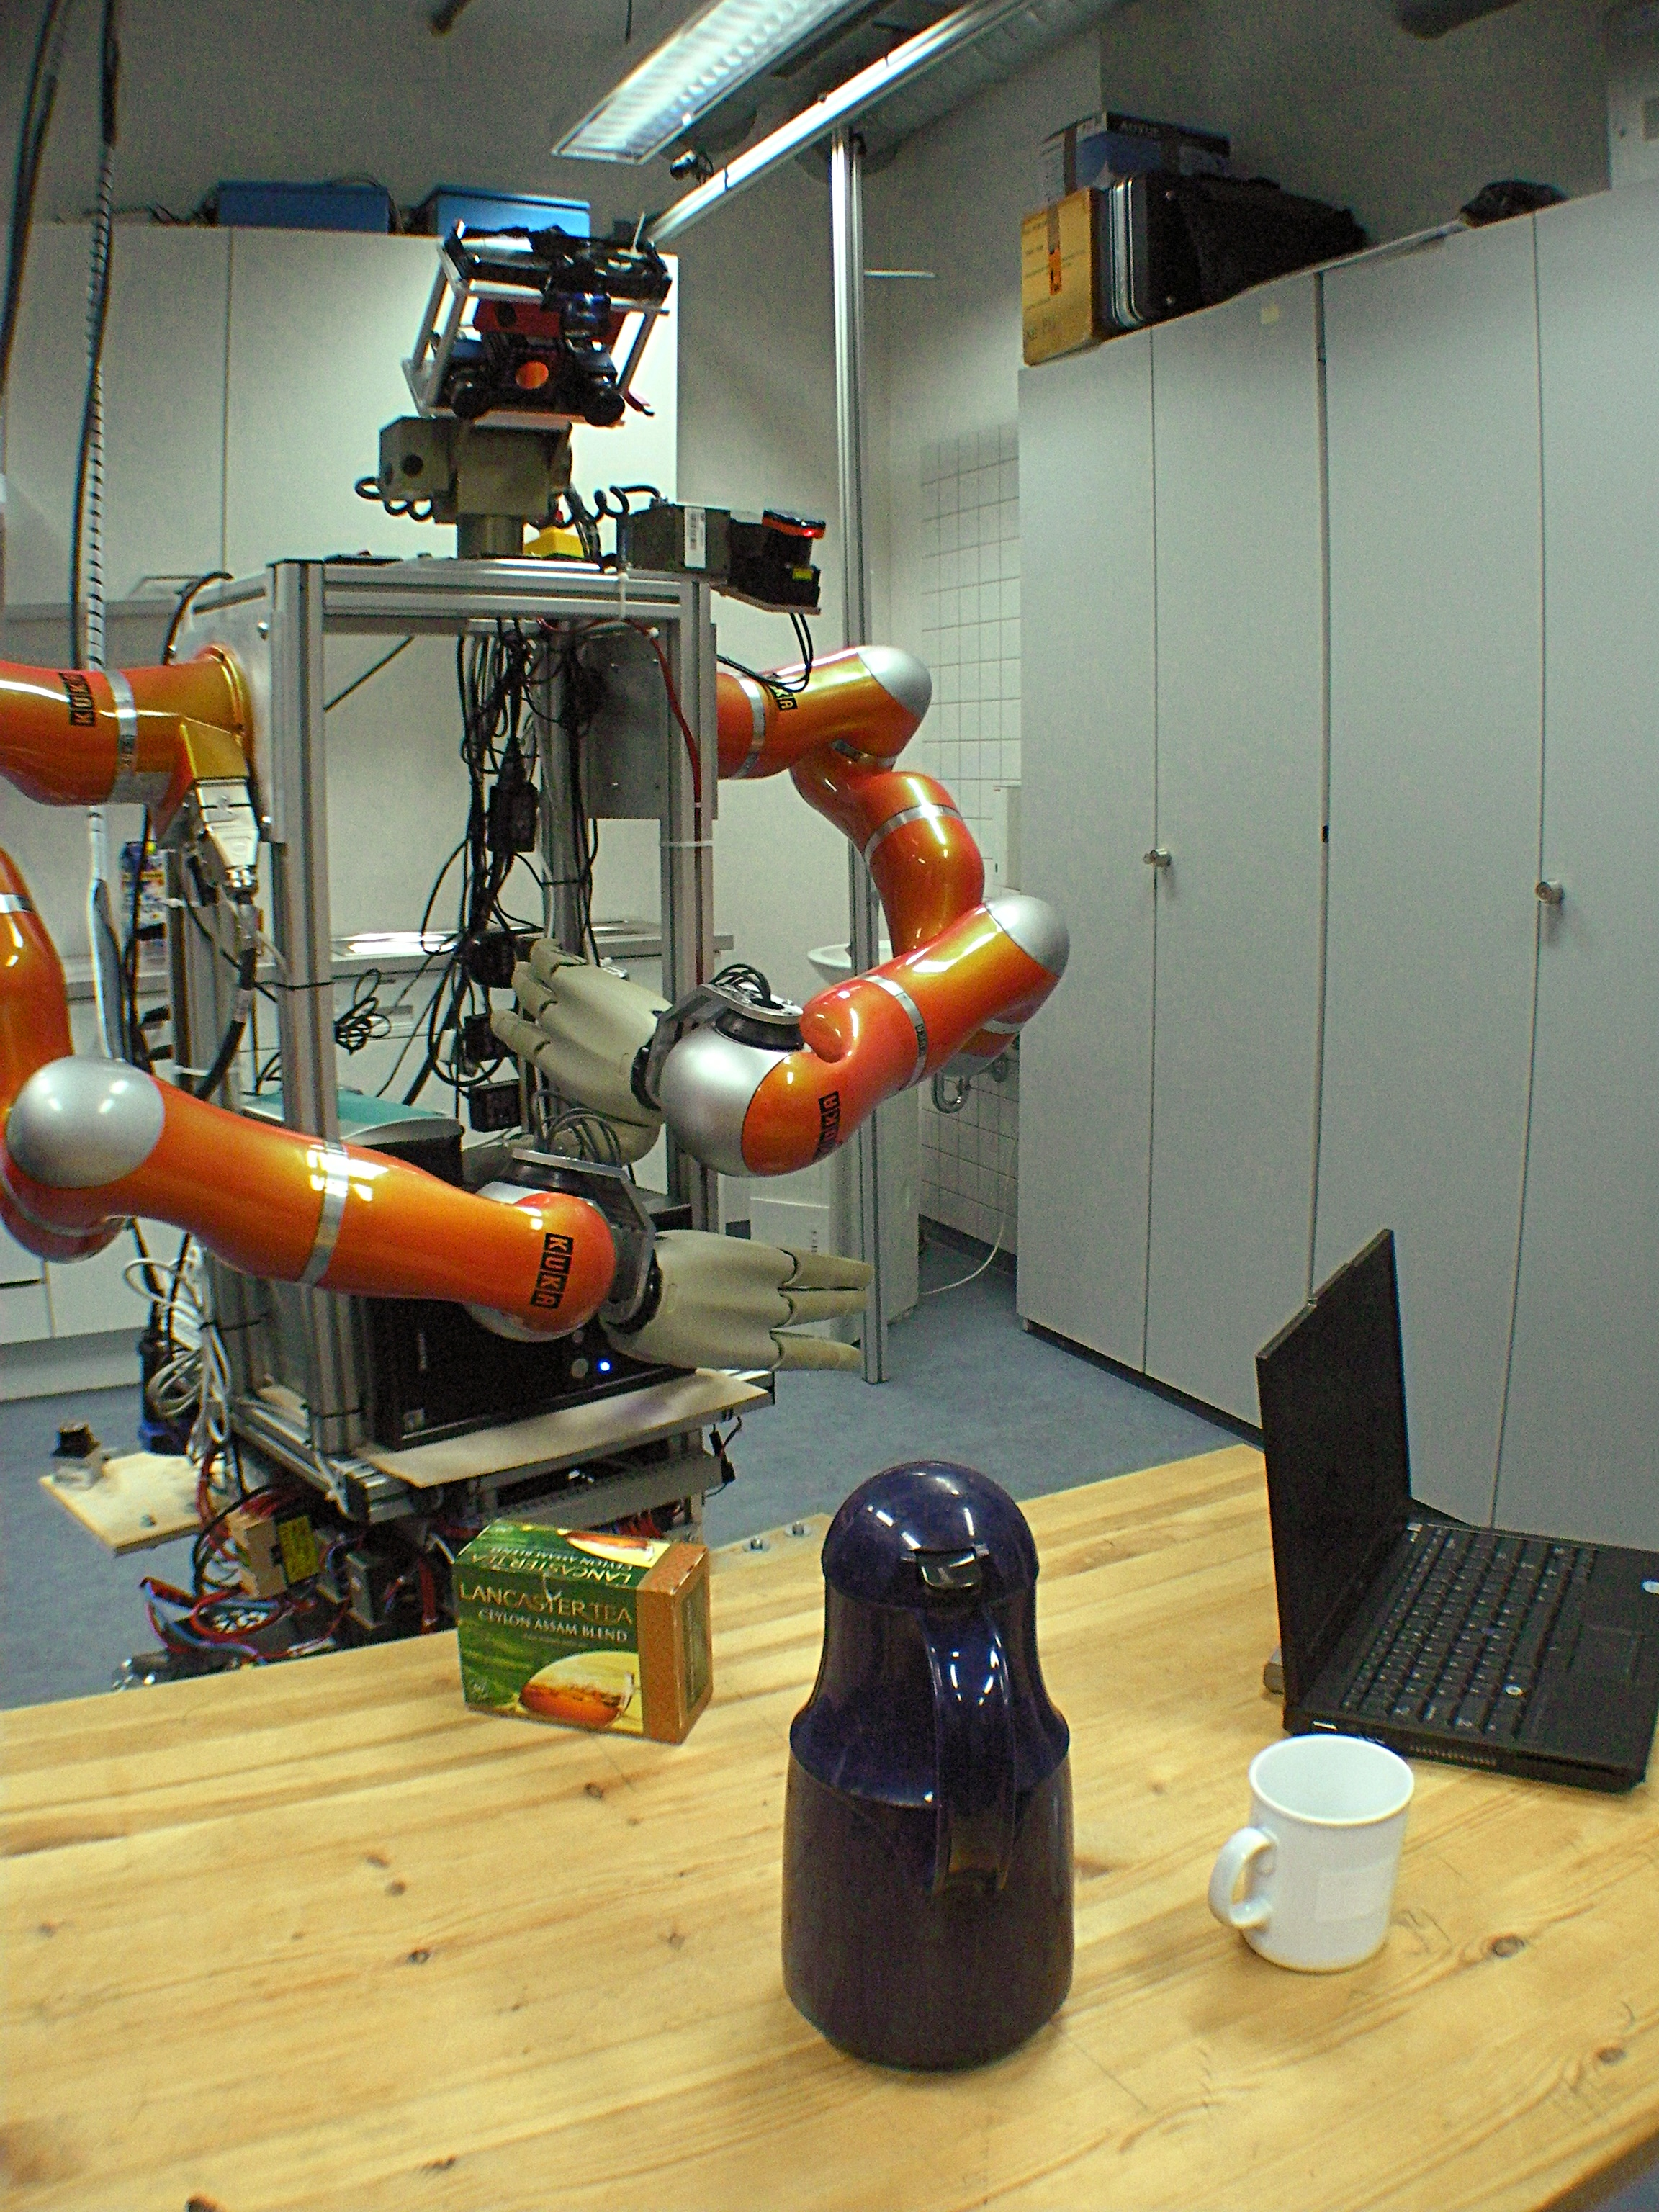
\includegraphics[width=0.45\columnwidth]{images/kimp1.jpg}
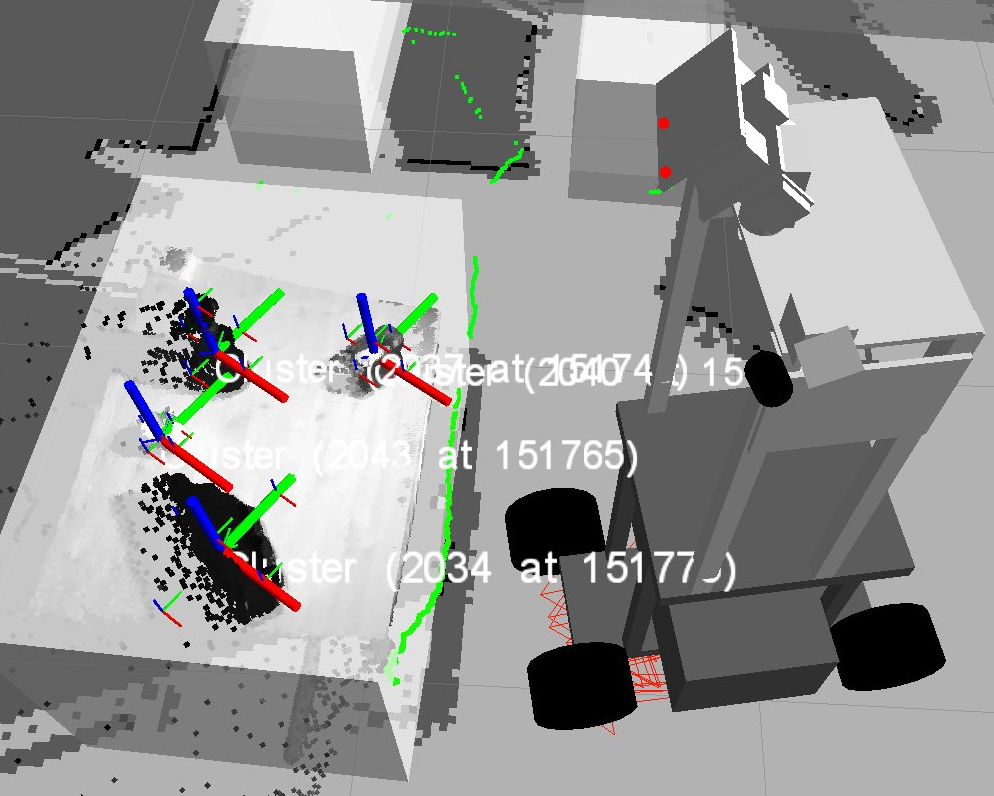
\includegraphics[width=0.45\columnwidth]{images/rviz.png}
%\parbox[c]{4.3cm}{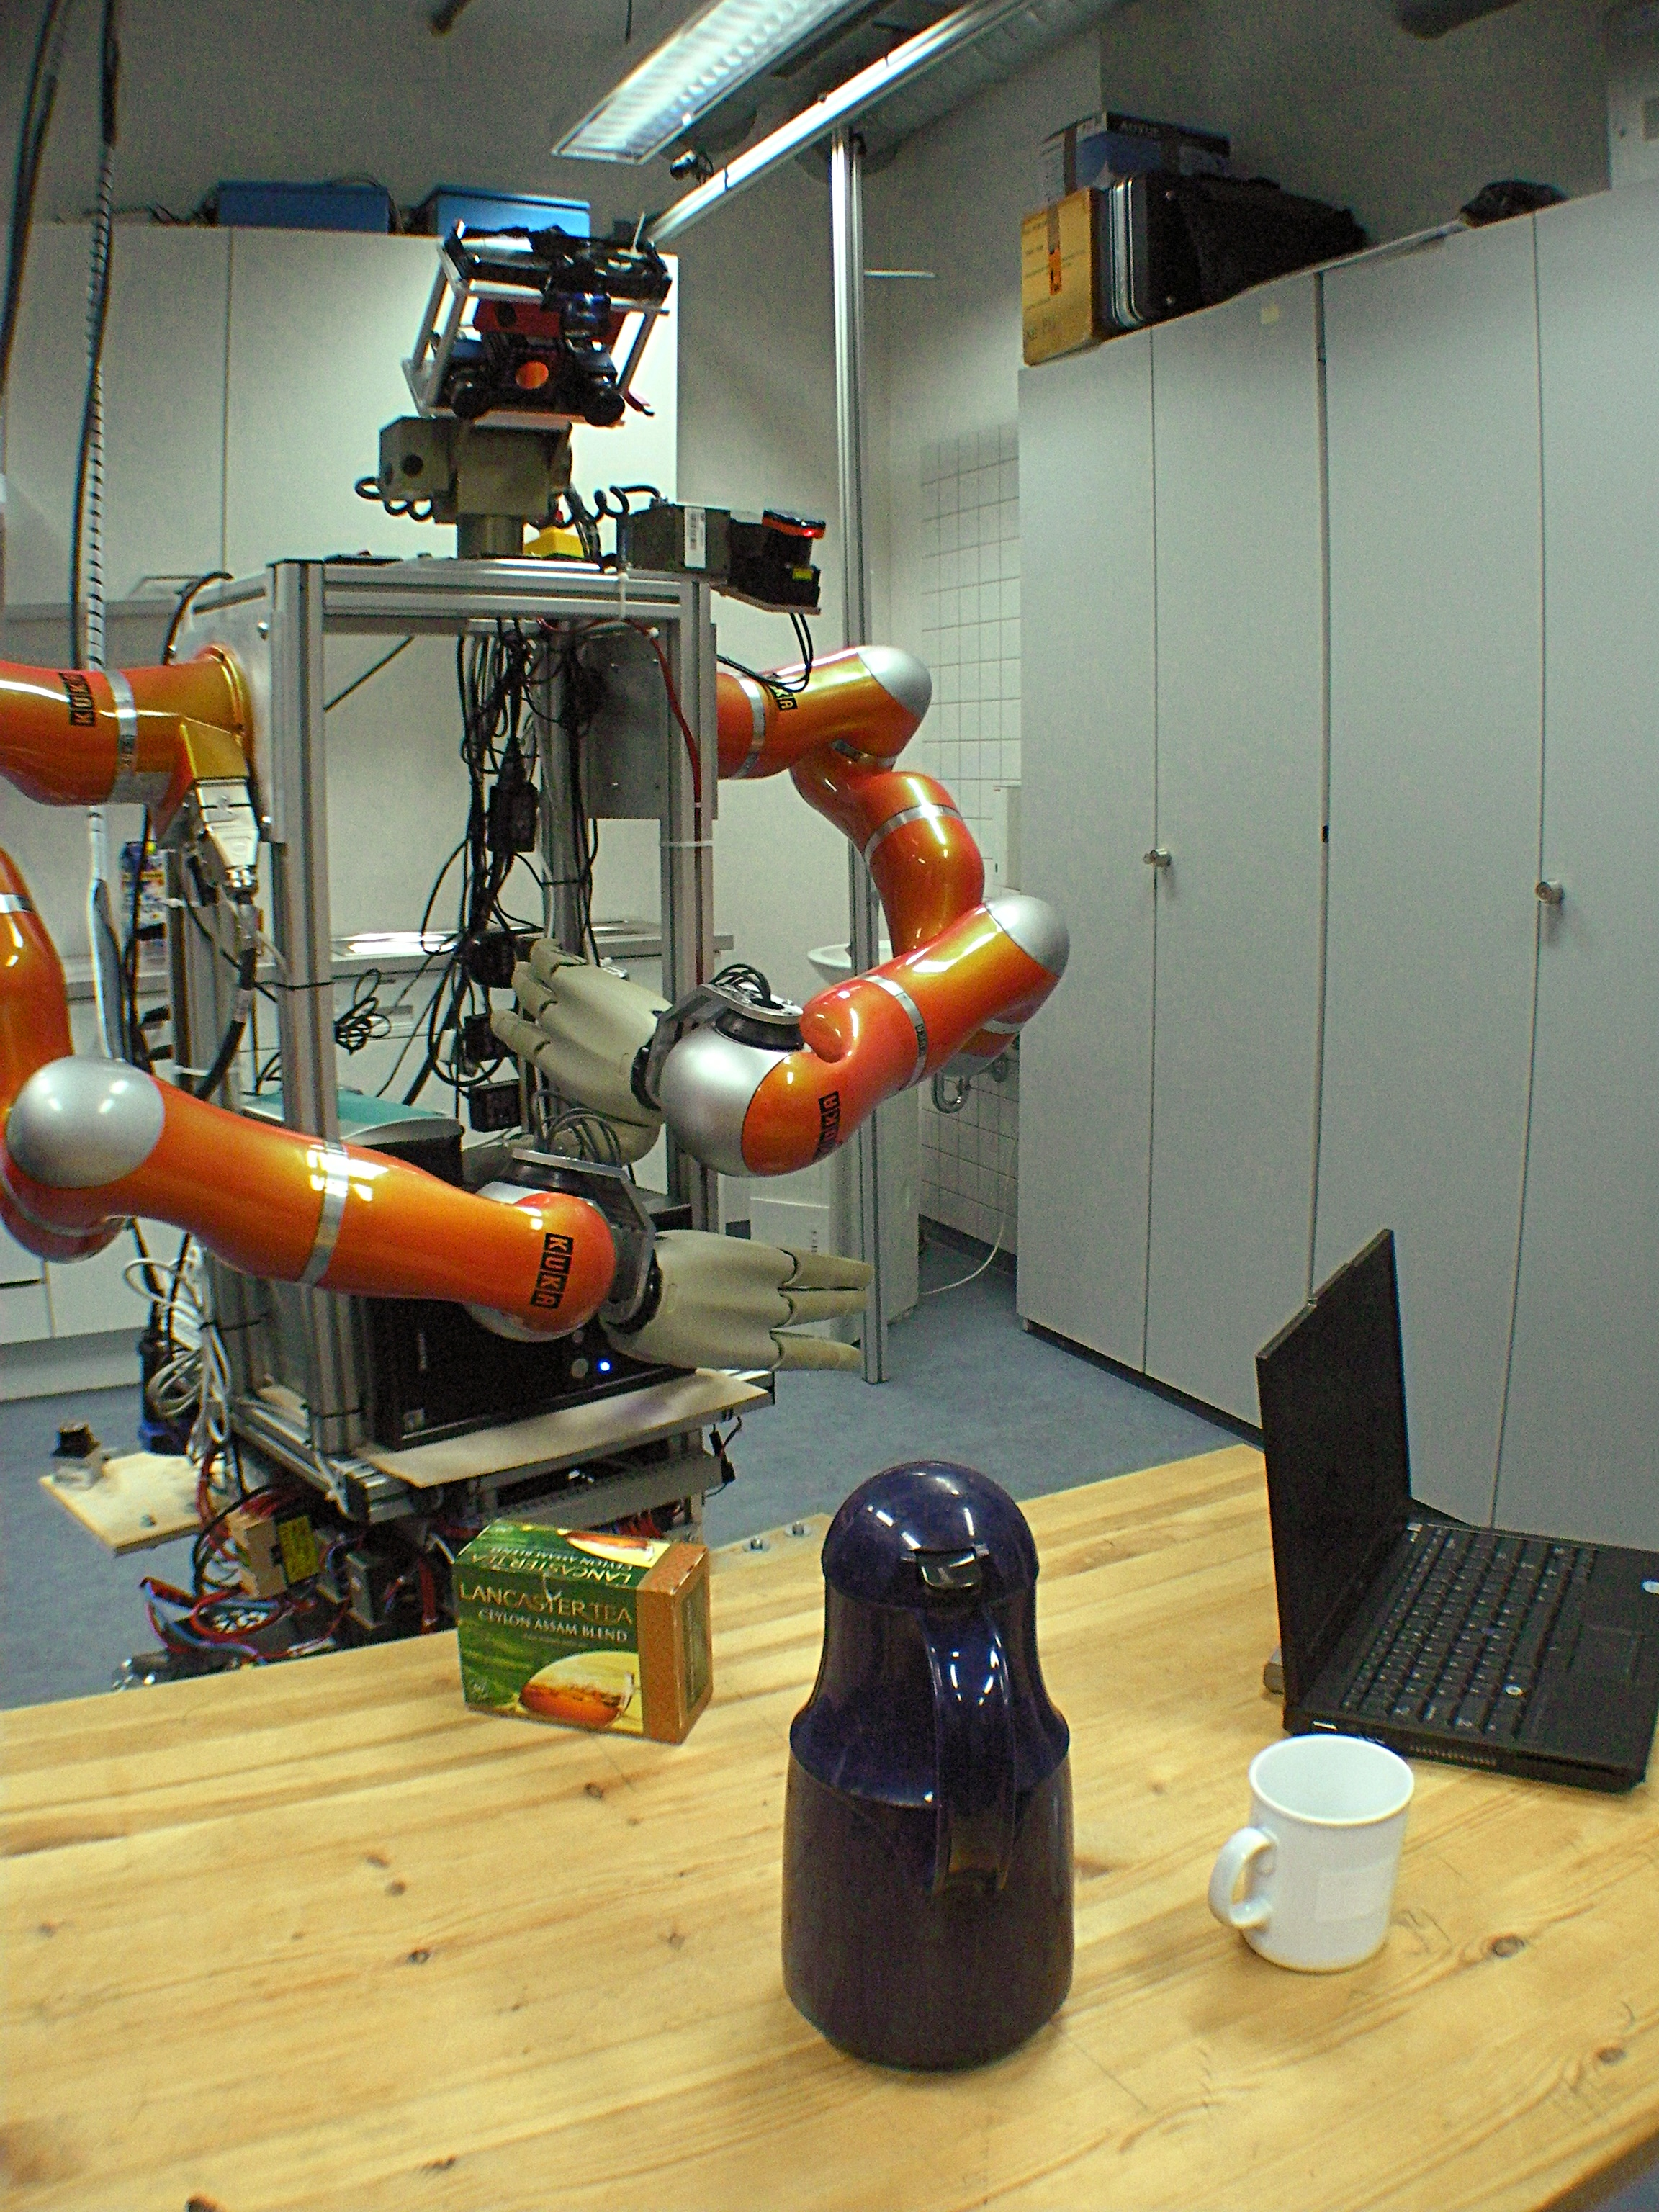
\includegraphics[width=0.5\columnwidth]{images/kimp1.jpg}}
%\parbox[c]{4.1cm}{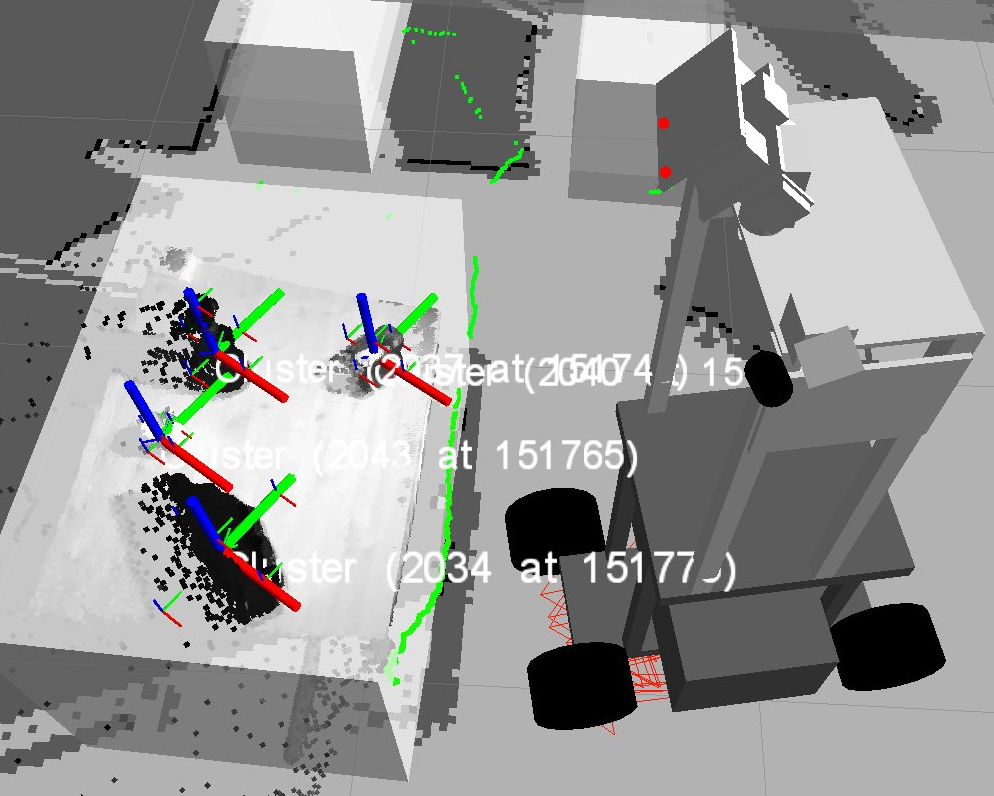
\includegraphics[width=4cm]{images/rviz.png}}
\flushleft
\hspace{1.8cm} (a) \hspace{3.9cm} (b)
\caption{(a) Rosie, looking for objects it may know, and (b) view from Willow
Garage's RViz. The clusters of point are given a unique identifier by the
perception that allows the supervision to create the link between the physical
objects and their symbolic representation in ORO.} 
\label{fig|kimpwatching}
\end{figure}

The \emph{Naming} task uses ORO to anchor perception into the robot's knowledge
through interaction with the user. This task has been implemented on the Rosie
robot at Munich university.

The robot selects an unknown object from the table, shows it to the user, and
asks about its name and type (Figure~\ref{fig|kimpwatching}). The user
interacts with the robot through a dedicated bridge, allowing him/her to chat with
the robot with a standard Jabber instant messaging client.
Figure~\ref{tab|transcript_kimp} shows a chat session with Rosie performing the
naming experiment. The human describes the object until the robot recognizes a
type it already knows. More precisely, the robot recursively asks the human for the categories the object belongs to until reaching a known one. At this point, the robot is able to connect the new object information to already known concepts. Therefore, the robot
accurately anchors perception in its symbolic model and it is able to reason
about it.  The learning process starts over again with each unknown object. To
further exploit the knowledge reasoner in this experiment, we ask the robot
which object do not belong to a typical breakfast table, \ie we ask for the odd
objects. In this case, it corresponds to objects that are neither of type
\concept{Tableware} nor \concept{Food}. 

The supervision module (\textsc{cram}\footnote{\textsc{cram} (Cognitive Robotic
Abstract Machine) is a RPL-derived framework for rapid development of cognitive
robot control programs we currently develop.}~\cite{Beetz2010}) automatically
updates the ORO server whenever an object enters or leaves the field of view.
%(the perception is based on the \textsc{CoP} framework~\cite{Klank2009}). 
Therefore, the integration of ORO can be seen as an extension of
the robot's belief state that not only contains abstract identifiers
of the internal object representation used in plans, but also the
semantics and roles of objects in the scenario.

\begin{figure}[!ht]
\centering
	\begin{tabular}{r|p{7cm}}
	\chatN{rosie} & Servus! The Bavarian robot is up and fit! \\
	\chatN{rosie} & What is the name of the white cluster on the table? \\
	\chatN{human} & ``Rosie's mug'' \\
	\chatN{rosie} &\emph{[\stmt{obj\_01 label "Rosie's mug"} added]}\\
				& What kind of object is ``Rosie's mug''? \\
	\chatN{human} & Mug \\
	\chatN{rosie} & \emph{[\stmt{obj\_01 type Mug} added]}\\
			& What is a Mug?\\ 
	\chatN{human} & Tableware\\
	\chatN{rosie} & \emph{[\stmt{Mug subClassOf Tableware} added. Rosie already
	knows about \emph{Tableware} (it belongs to the common-sense ontology), so
	the interaction stops.]}\\
	& (...) \\
	\chatN{rosie} &  What is the name of the black cluster on the table? \\
	\chatN{human} & ``my\_laptop'' \\
	\chatN{rosie} & What kind of object is ``my\_laptop''? \\
	\chatN{human} & Computer \\
	\chatN{rosie} & What is a Computer? \\
	\chatN{human} & Artifact \\
	\chatN{rosie} & Do you want me to learn more objects? \\
	\chatN{human} & no \\
	\chatN{rosie} & These objects are odd: ``my\_laptop'' \\
	\end{tabular}
	\caption{Transcript of a Jabber session with the robot Rosie.}
	\label{tab|transcript_kimp}
\end{figure}

An unexpected example of what the symbolic reasoning layer brings to more
traditional robotic architectures emerged during the \emph{Naming} experiment:
the perception routines provided segmented blobs corresponding to objects along
with their colors to update the information in ORO. At some point, ORO suddenly
refused to add an object. What seemed at first a communication bug between
modules, was actually the consequence of a consistency check by ORO: because of
bad light conditions, the color recognition was not very reliable, and the same
object was set to have two different colors at the same time. Since the
\concept{hasColor} predicate we had decided to use was a functional predicate
(\ie objects can have only one color), ORO inferred an inconsistency and
discarded the new fact. This kind of logical failure can be used to improve
low-level perception outcomes by ``closing the loop'' with high-level, symbolic
knowledge.

\subsection{\emph{Spy Game} experiment}

\label{spygame}

This game is based on the traditional children game ``I Spy''. The idea is to
discover the object or concept one of the participants is thinking of by asking
questions such as: ``Is it green? Is it a machine? Is it on your left?'', etc.
When playing, children exploit their knowledge about the world while
categorizing and describing objects through useful discriminants that will
allow them to find out the answer as fast as possible while including
perspective taking abilities~\cite{Moll2006}.

\begin{figure}
\centering
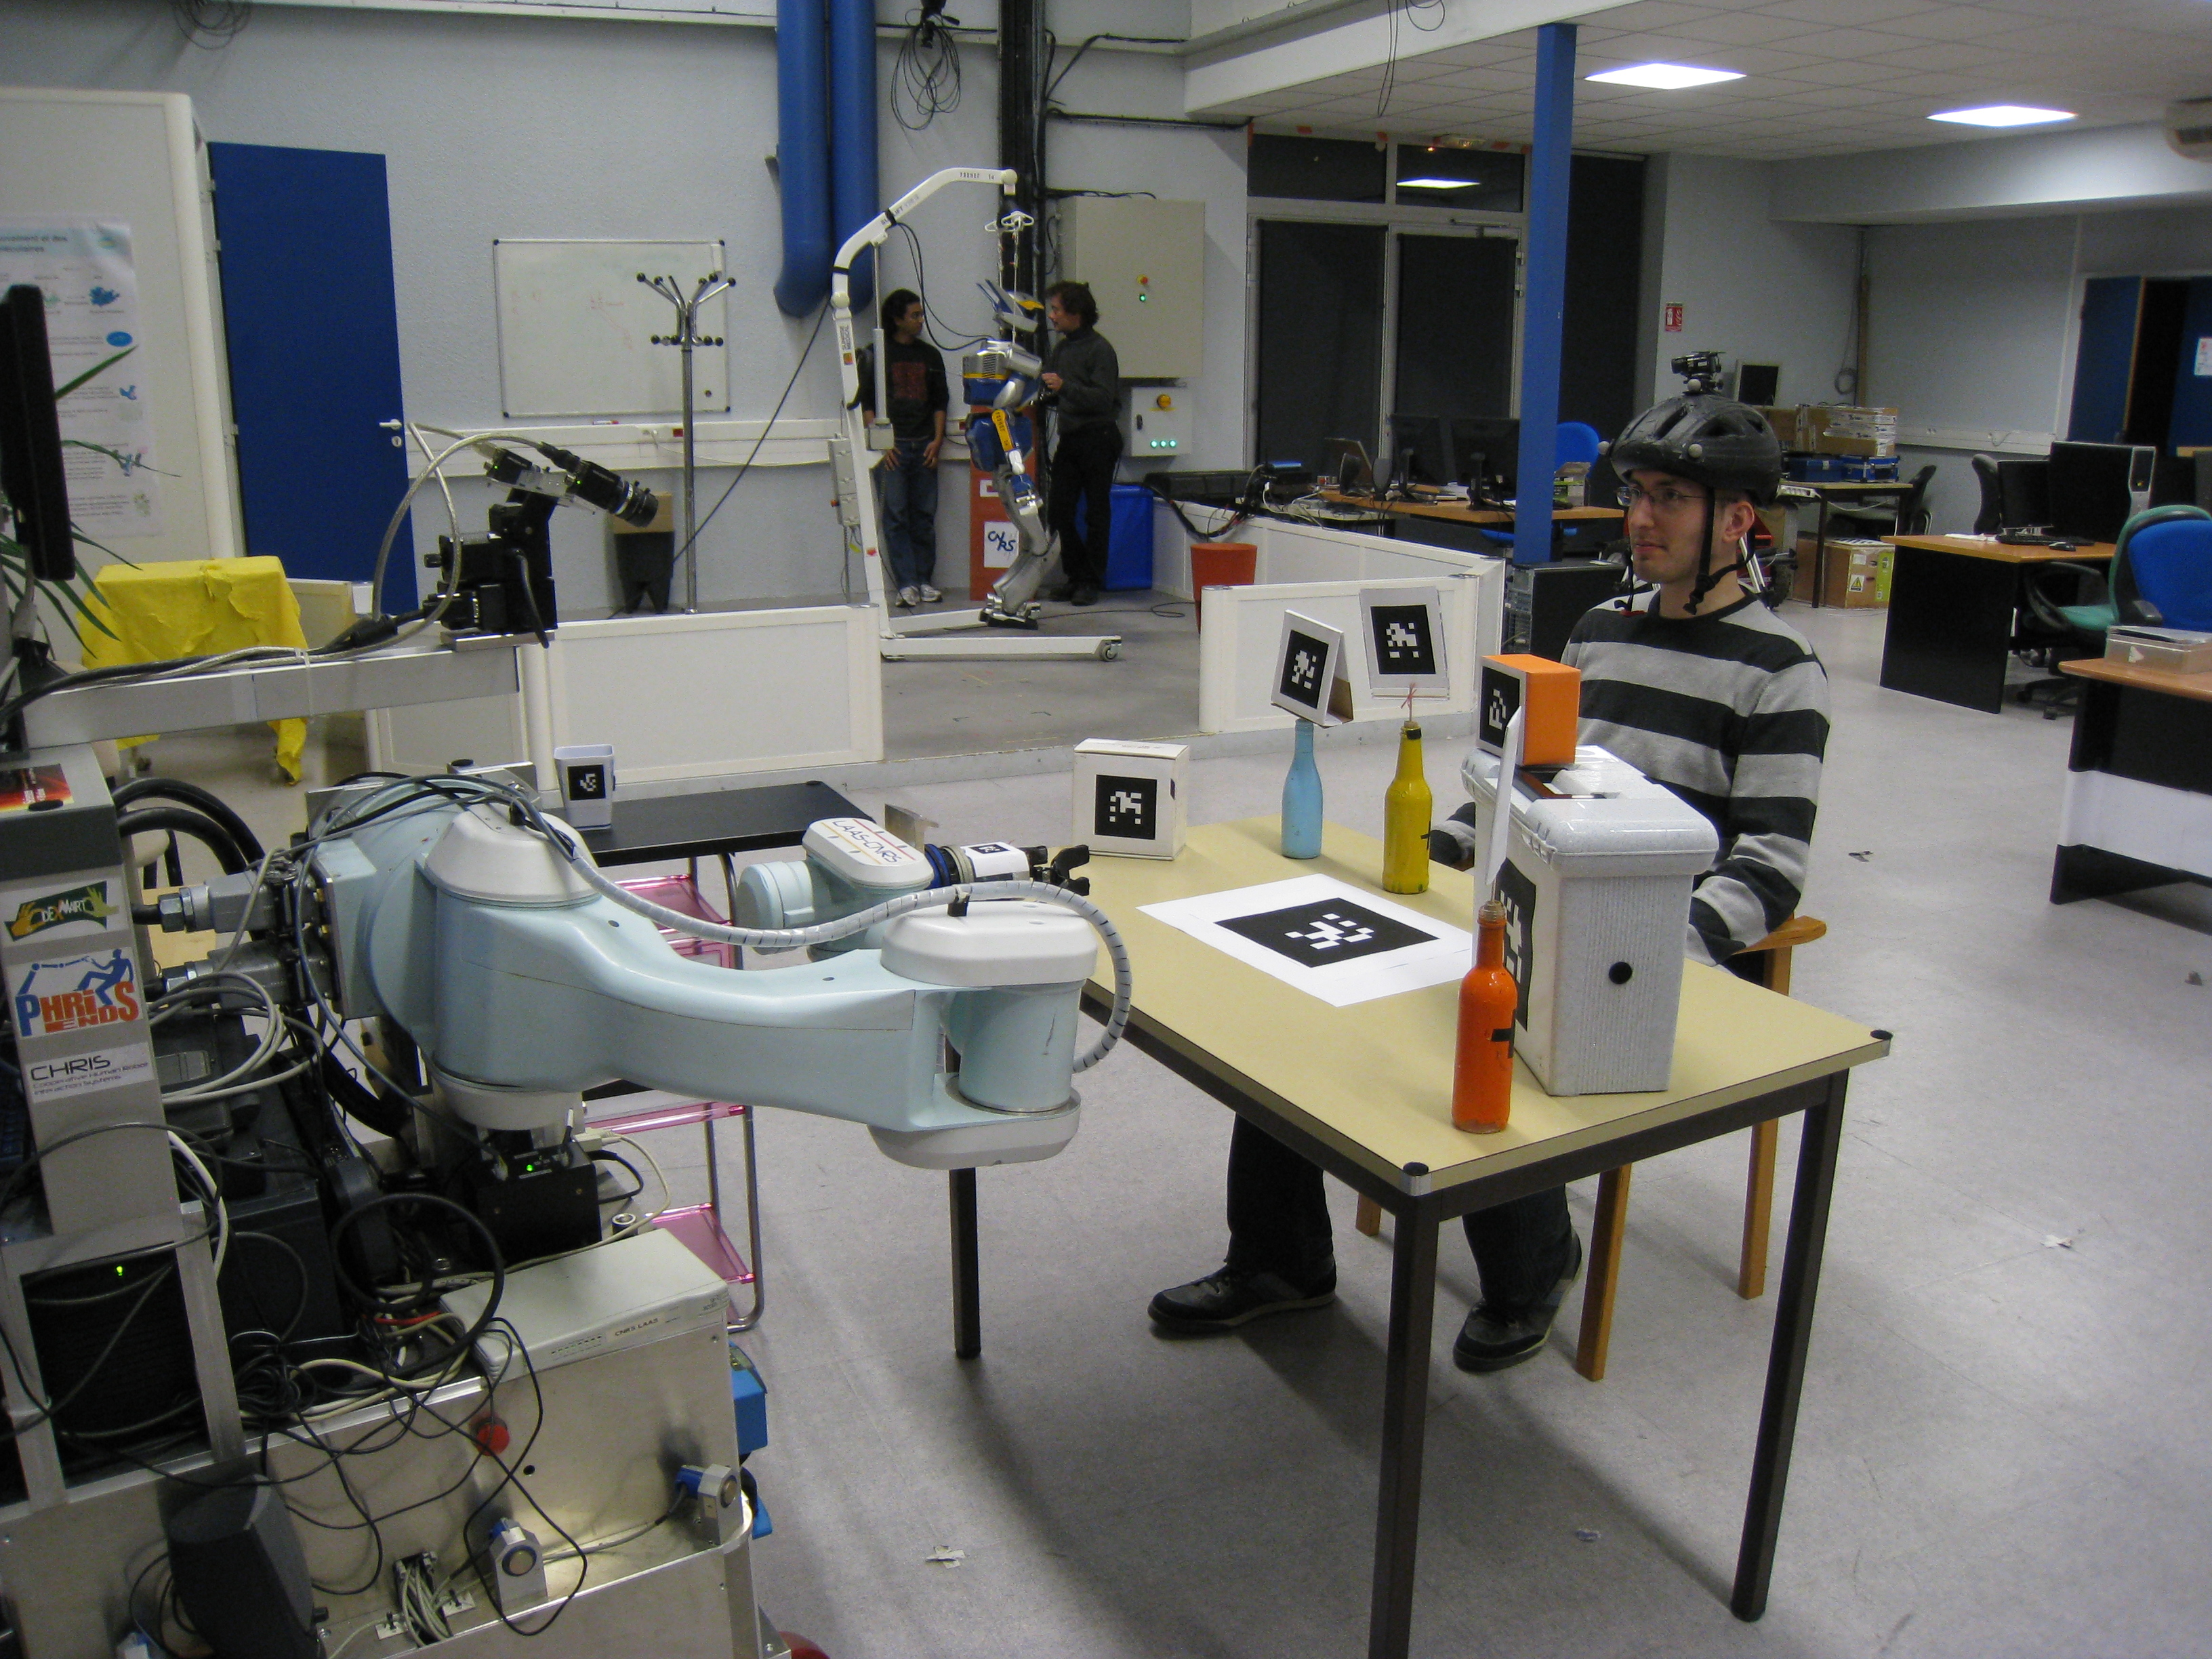
\includegraphics[width=0.45\columnwidth]{images/spy-game-real.jpg}
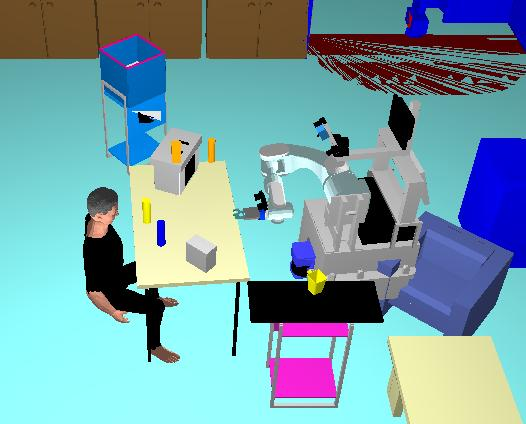
\includegraphics[width=0.45\columnwidth]{images/spy-game-mhp.jpg}
%\parbox[c]{4.3cm}{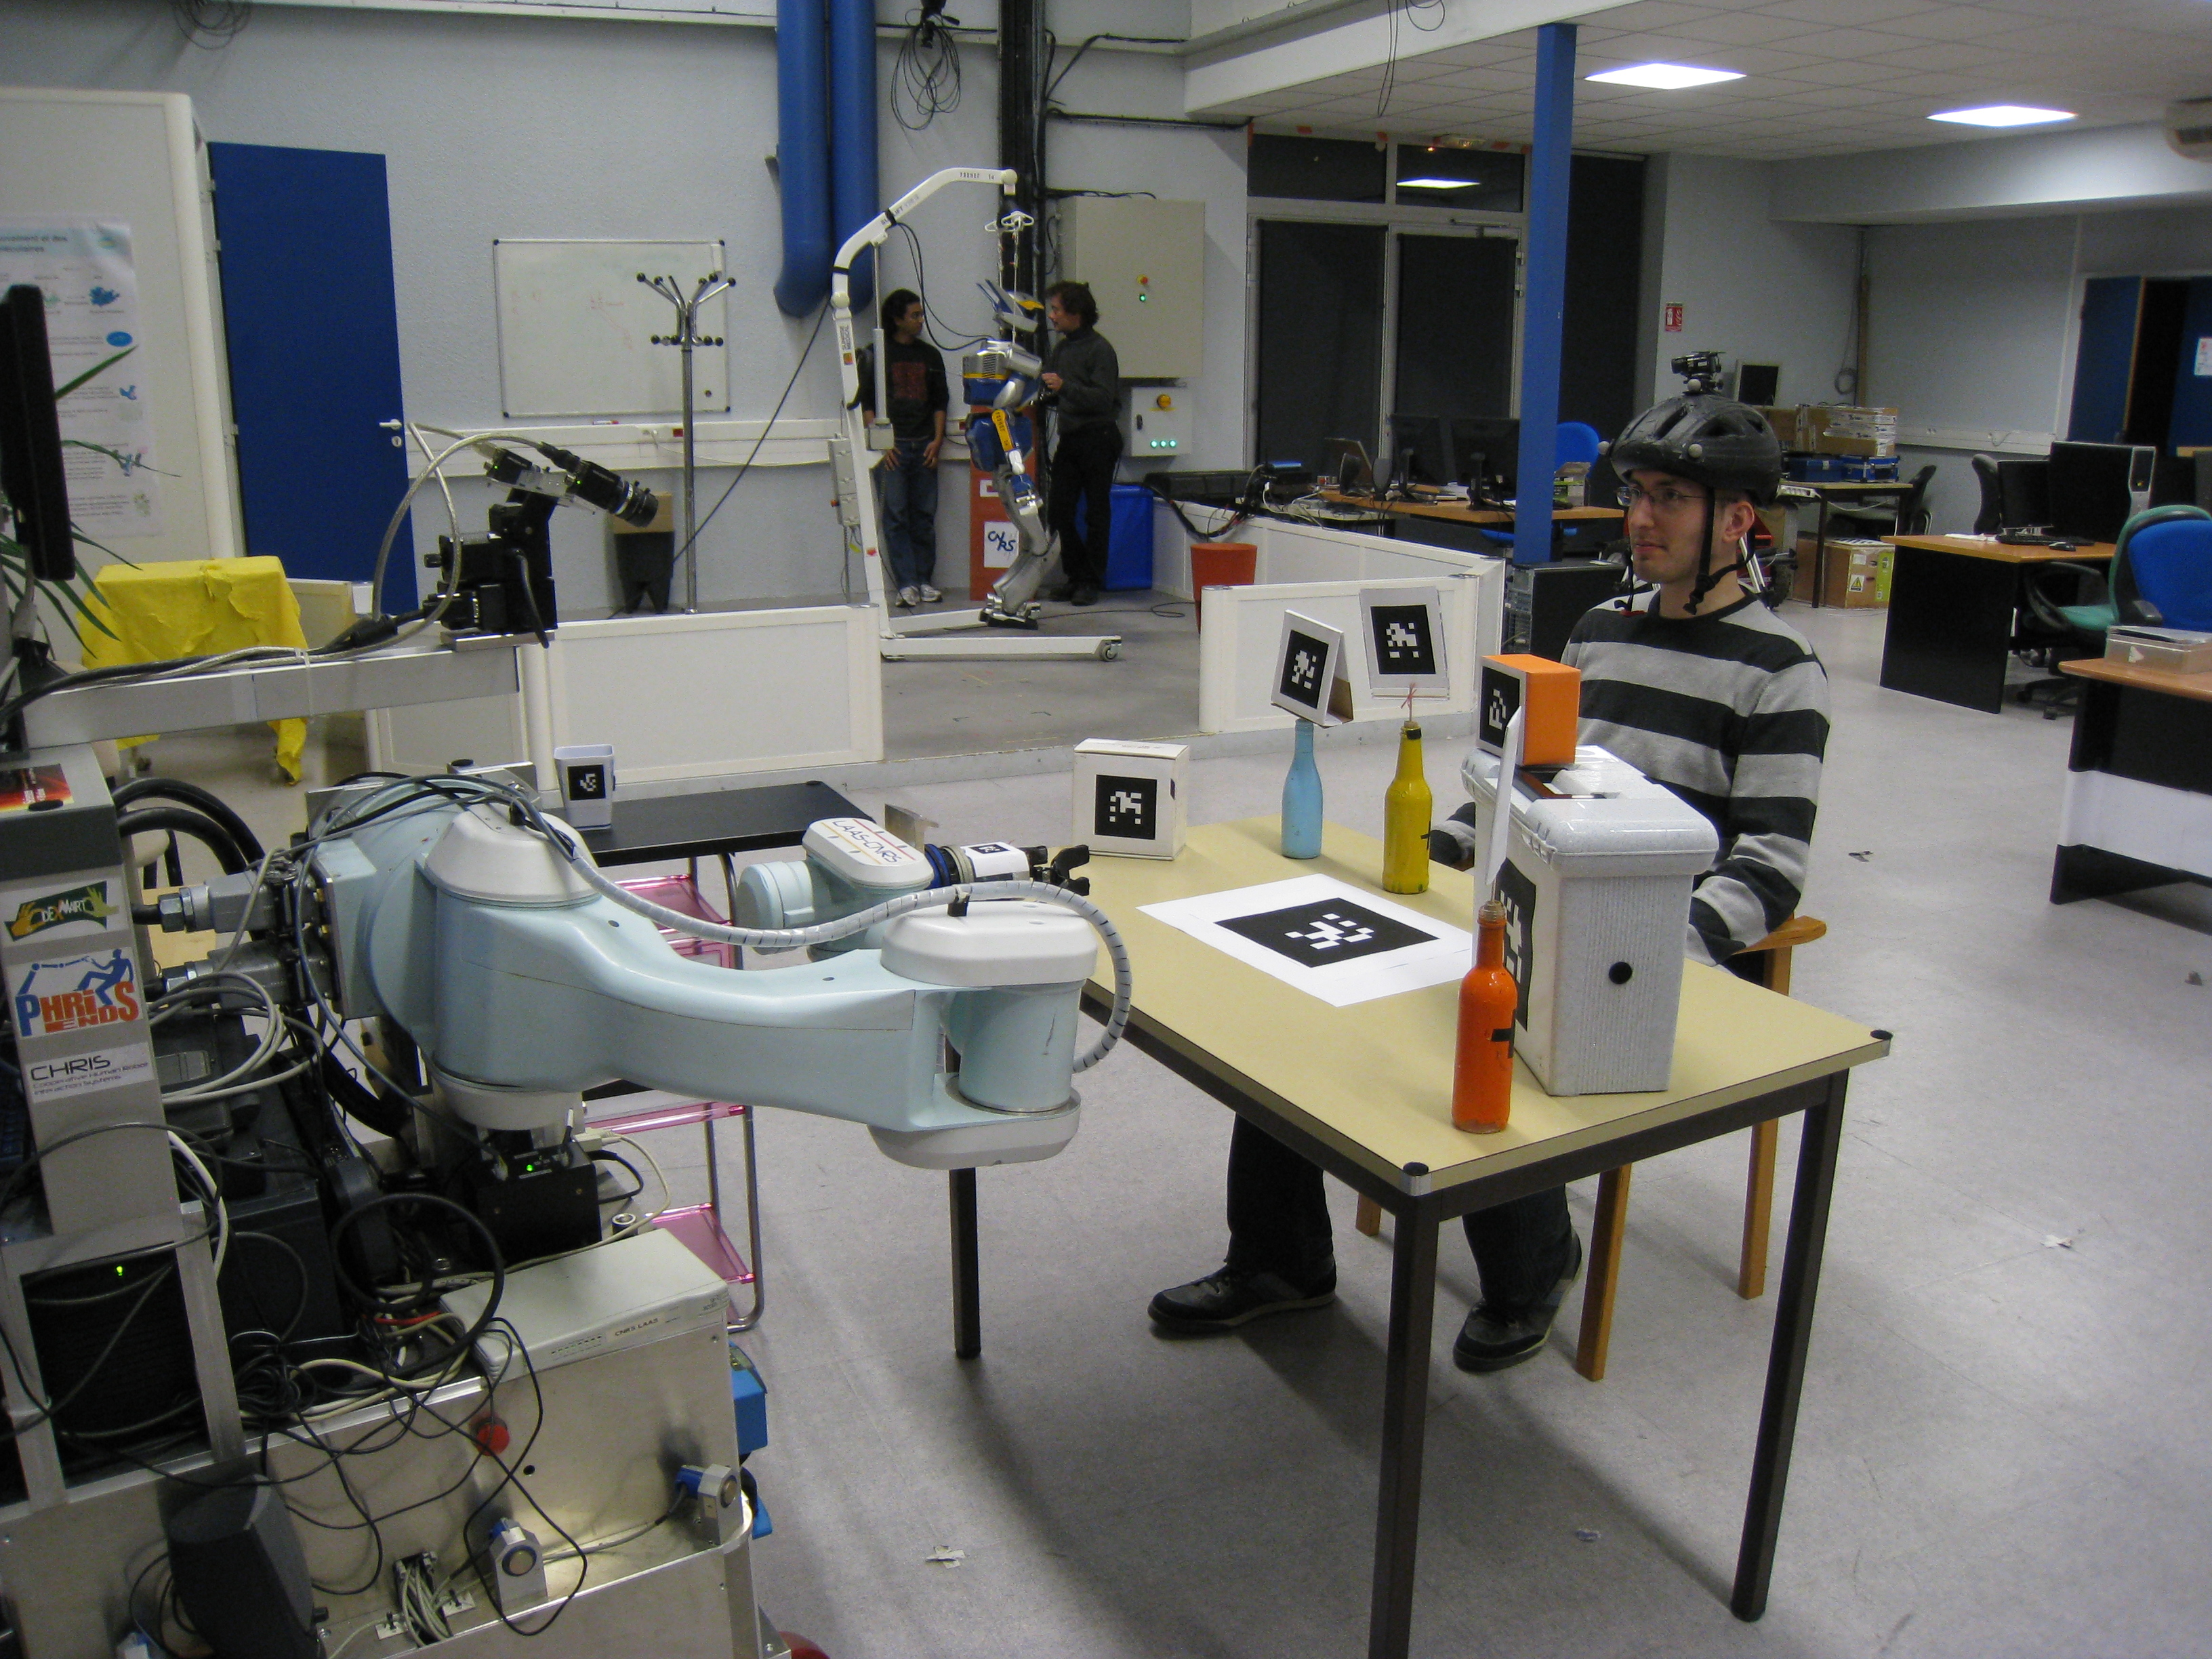
\includegraphics[width=4.3cm]{images/spy-game-real.jpg}} \hspace{0.2em}
%\parbox[c]{4.1cm}{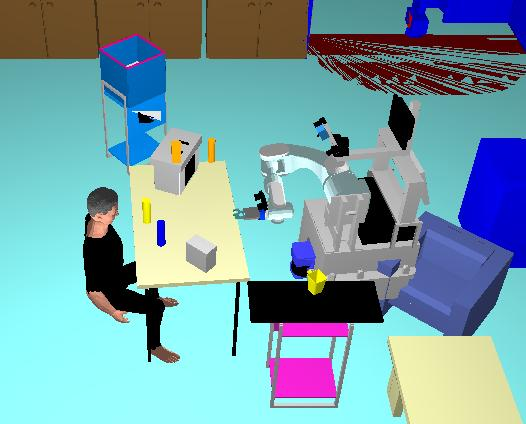
\includegraphics[width=4.1cm]{images/spy-game-mhp.jpg}}
\flushleft
\hspace{1.8cm} (a) \hspace{3.9cm} (b)
\caption{Spy game scenario: (a) Real environment and (b) 3D environment model, viewed in \textsc{SPARK}.}
\label{fig|spyGameScenario}
\end{figure}

The scenario for this game (Figure~\ref{fig|spyGameScenario}) consists on a
face-to-face interaction where the human thinks of an object present in the
environment, while the robot queries the human until either discovering the
object or giving up~\cite{Ros2010a}. A categorization example is presented in
Figure~\ref{fig|objectsSpyGame}. The game starts with the human user giving a
first hint (communication is done through a keyboard and screen), allowing the
robot to start the search filtering those objects that fulfill this first
description. Based on this subset, ORO provides a descriptor (or set of
descriptors) that allows a maximum discrimination among objects in the subset.
The robot queries the user about the value of the descriptor (or the most
discriminant among the set of descriptors) and with this new information, the
current subset of objects is filtered again. The process is repeated until
either obtaining a single object that fulfills all the descriptor values, or
failing (\ie no object found). 

\begin{figure}[!ht]
\centering
\begin{scriptsize}
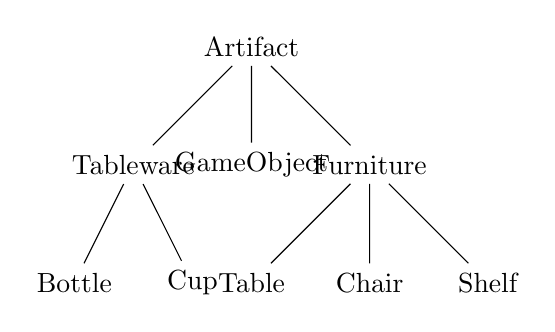
\begin{tikzpicture} %[level/.style={sibling distance=30mm/#1},scale=0.8]
	%[edge from parent fork down,
	%every node/.style={fill=black!30,rounded corners},
	%[parent anchor=east,child anchor=west,grow=east,
	%edge from parent/.style={thick,draw}]
	\node {Artifact}
	child {node {Tableware}
		child {node {Bottle}}
		child {node {Cup}}
		}
	child {node {GameObject}}
	child {node {Furniture}
			child {node {Table}}
			child {node {Chair}}
			child {node {Shelf}}};
\end{tikzpicture}
\end{scriptsize}
\caption{Example of object categorization used in the scenario.}
\label{fig|objectsSpyGame}			
\end{figure}

%Thing
%Object
%Tableware
%	- bottle: red, blue, yellow orange
%	- cup: white
%Furniture
%	- table: hrp2table, lowtable
%	- chair: chair1 and chair2
%	- shelf: pink_shelf
%GameObject: spacenavbox, orangebox, accesskit

We have integrated the game on the LAAS-CNRS Jido robot.
Objects are identified through a tag-based vision approach\footnote{ARToolKit:
\url{http://www.hitl.washington.edu/artoolkit/}} and motion capture is used for
human tracking. Their descriptions regarding categories (type of object) and
features (color, shape) are manually given in advance. Spatial relationships
(\concept{front}, \concept{back}, \concept{left}, etc, and \concept{in},
\concept{on} and \concept{next to}) and visibility (only visible objects for
both agents can be considered in the game) are automatically computed on-line
by \textsc{SPARK} (the geometric reasoner). Figure~\ref{fig|spyGameExample}
shows an example of a round game.


\begin{figure}
\centering
	\begin{tabular}{r|p{6cm}}
		\chatN{human} & It is a tableware.\\
		\chatN{jido} & \emph{[retrieve possible objects: coke-bottle, yellow-bottle, orange-bottle, cup-with-handle]} \\
	 			& \emph{[keep visible objects: coke-bottle, yellow-bottle, cup-with-handle]}\\
				& \emph{[obtain discriminants: type, color.]}\\
				& Which type of object is: bottle or cup? \\
		\chatN{human} & Bottle.\\
		\chatN{jido} & \emph{[obtain possible objects: coke-bottle, yellow-bottle.]}\\
				& \emph{[obtain discriminants: color.]}\\
				& What color is the object: red or yellow?\\
		\chatN{human} & Red.\\
		\chatN{jido} & \emph{[obtains possible objects: coke-bottle.]}\\
				& The object is the Coke bottle!	
	\end{tabular}\\
	\caption{Example of the robot playing Spy game.}
	\label{fig|spyGameExample}
\end{figure}

\subsection{``Moving to London'' scenario}

In order to illustrate some of different reasoning abilities of the robot presented in this paper, we have designed the following
daily life situation. Tom and Jerry are moving to London, so they are packing
things in boxes. The scenario takes places in the living-room, where Jido (our
robot) is observing while they move things here and there. To assess the
reasoning abilities of the robot they ask Jido for information (entered through
keyboard). Ideally, the robot should also perform actions when required (\eg
hand an object when asking ``give me...''). However, since it is out of the
scope of this work, we do not include any motion from the robot's side. Similar
to the \emph{Spy Game} scenario, perception of objects is done through a tag-based
system and humans are detected through motion capture. We next describe in
detail three situations where we can follow the internal robot's reasoning and
the interaction with the users.

\subsubsection{Initial situation assessment}

\begin{figure}[!t]
\centering
  \subfigure[]
  {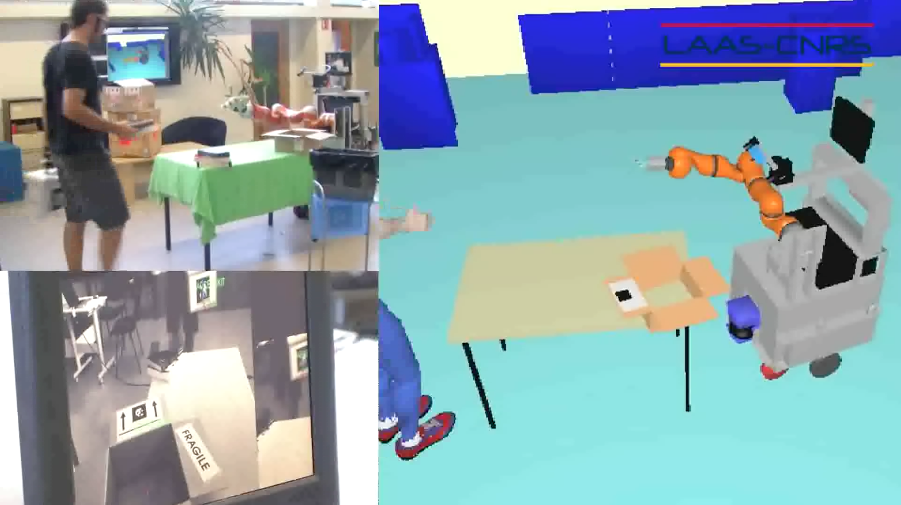
\includegraphics[width=0.95\linewidth]{images/situationAssessment1.png}\label{a}}
  \subfigure[]
  {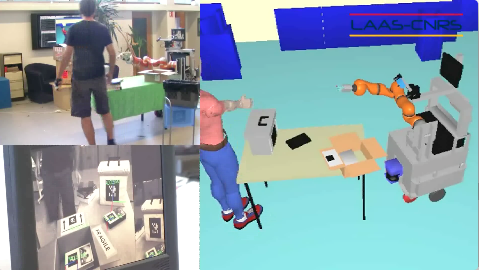
\includegraphics[width=0.95\linewidth]{images/situationAssessment2.png}\label{b}}
	\caption{Situation assessment during initialization: a) before placing the
	objects on the table, and b) after placing them. In each image the snapshots
	correspond to: real environment (top-left sub-image); processed image to
	identify the tagged objects (bottom-left sub-image); and the 3D environment
	(right sub-image).}
	\label{fig|sitAssessRoman}
\end{figure}

First Tom enters the room with some of the things they need to pack: a
toolbox and two videos. He leaves one of the videos (``Jido-E'') inside one of
the boxes (the cardboard box), and the other one (``Lord of the Robots'') on the
table. We next describe how the situation assessment takes place, \ie how the
ontology is updated with the information obtained from the geometric reasoner
SPARK.

The initial information in ORO corresponds to:

\begin{center}
    \begin{tabular}{l}
      \stmt{table type Table}\\
      \stmt{cardBoardBox type Box}\\
      \stmt{toolbox type Box}\\
      \stmt{videoTape1 type VideoTape}\\
      \stmt{videoTape1 label "Lord of the Robots"}\\
      \stmt{videoTape2 type VideoTape}\\
      \stmt{videoTape2 label "Jido-E"}\\
      \stmt{Tom type Human}\\
      \stmt{Jerry type Human}
    \end{tabular}
\end{center}
\vspace{0.10cm}
	
SPARK detects that there is a cardboard box on the table. It thus sends the fact to ORO:

\begin{center}
    \begin{tabular}{l}
      \stmt{cardBoardBox isOn table}
    \end{tabular}	             
\end{center}

Tom enters carrying several objects (Figure~\ref{fig|sitAssessRoman}a).
He places a toolbox and a video tape on the table, and another video tape
inside the box next to Jido and the leaves. (Figure~\ref{fig|sitAssessRoman}b). The following facts are computed and sent to ORO:

\begin{center}
    \begin{tabular}{l}
      \stmt{toolbox isOn table}\\
      \stmt{videoTape1 isOn table}\\
      \stmt{videoTape1 isNextTo toolbox}\\
      \stmt{toolbox isNextTo videoTape1}\\
      \stmt{videoTape2 isIn cardBoardBox}
    \end{tabular}       
\end{center}

\subsubsection{Implicit disambiguation through visual perspective taking}

Tom enters the room again while carrying a big box (Figure~\ref{fig|vpt}). He
approaches the table and asks Jido to handle him the video tape: ``Jido, can
you give me the video tape''. The \textsc{Dialogs} module queries the ontology to
identify the object the human is referring to:

\begin{center} 
\stmt{?obj type VideoTape} 
\end{center}

There are two video tapes in the scene: one on
the table, and another one inside the cardboard box. Thus, the knowledge 
base returns both: 

\begin{center}
\hspace{0.7cm}$\Rightarrow$ \concept{?obj = [videoTape1, videoTape2]}
\end{center}

However, only one is visible for Tom (the one on the
table). Thus, although there is an ambiguity from the robot's perspective
(since it can see both video tapes), based on the perspective of its human
partner it infers that Tom is referring to the video tape on the table, and not
the one inside the box which is not visible from his view. Therefore,
non-visible objects are removed obtaining:

\begin{center}
\concept{?obj = [videoTape1]}
\end{center}

Since only one object is available now, the robot infers
that the human refers to it and can eventually execute the command, \ie give
it to the human. Alternatively, the robot could first verify with the human if
that was the object being referred to or not before proceeding to execute the
action. Table~\ref{table|ptbeliefs} lists the robot's beliefs about itself and
its human partner involved in this situation.

\begin{table}
\begin{center}
\begin{tabular}{l}
\hline
Robot's beliefs about itself (\emph{robot's model}):\\
\hline
  \hspace{0.7cm}\stmt{videoTape1 type VideoTape}\\
  \hspace{0.7cm}\stmt{videoTape1 isOn table}\\
  \hspace{0.7cm}\stmt{videoTape1 isVisible \textit{true}}\\
  \hspace{0.7cm}\stmt{videoTape2 type VideoTape}\\
  \hspace{0.7cm}\stmt{videoTape2 isIn cardBoardBox}\\
  \hspace{0.7cm}\stmt{videoTape2 isVisible \textit{true}}\\
\hline
\hline
Robot's beliefs about Tom (\emph{Tom's model}):\\
\hline
  \hspace{0.7cm}\stmt{videoTape1 type VideoTape}\\
  \hspace{0.7cm}\stmt{videoTape1 isOn table}\\
  \hspace{0.7cm}\stmt{videoTape1 isVisible \textit{true}}\\
  \hspace{0.7cm}\stmt{videoTape2 type VideoTape}\\
  \hspace{0.7cm}\stmt{videoTape2 isIn cardBoardBox}\\
  \hspace{0.7cm}\stmt{videoTape2 isVisible \textit{false}}\\
 \hline
\end{tabular}
\end{center}
\caption{Robot's beliefs about itself and its human partner.}
\label{table|ptbeliefs}
\end{table}

\subsubsection{Explicit disambiguation through verbal interaction and gestures}
\begin{figure}[!ht]
  \centering
  \subfigure[]
  {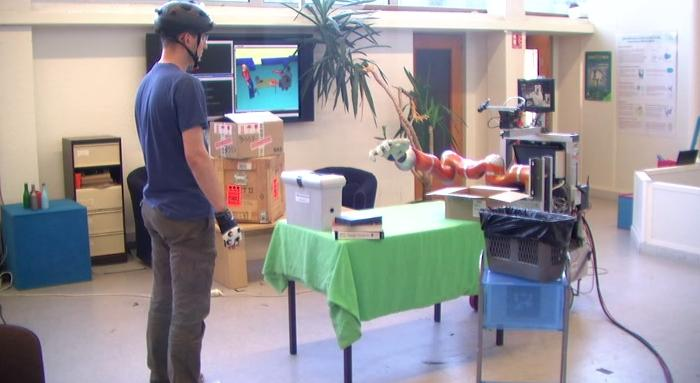
\includegraphics[width=0.9\linewidth]{images/inTheBox1.jpg}\label{a}}
  \subfigure[]
  {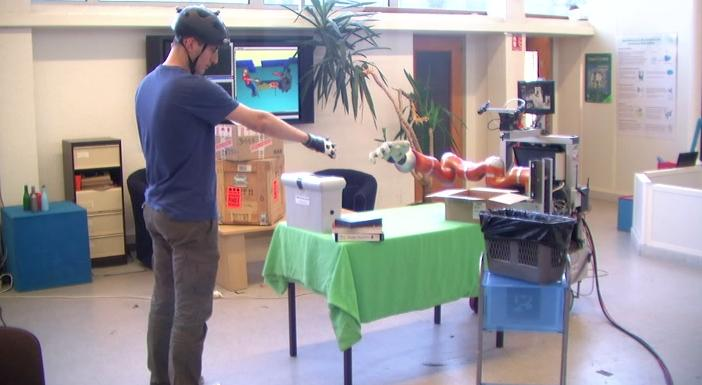
\includegraphics[width=0.9\linewidth]{images/inTheBox2.jpg}\label{b}}
\caption{(a) Jerry asks Jido for the content of the box and (b) points at it.}
  \label{fig|pointing}
\end{figure}

Figure~\ref{fig|pointing}a depicts the third situation where Jerry enters the
living room without knowing where Tom had placed the video tapes. So he first
asks Jido: ``What's in the box?''. Before the robot can answer the question it
has to figure out which box Jerry is talking about. Similar to the previous
situation, there are two available boxes: 

\begin{center}
\begin{tabular}{l}
\stmt{?obj type Box}\\
\hspace{0.7cm}$\Rightarrow$ \concept{?obj = [cardBoardBox, toolbox]}
\end{tabular}
\end{center}

However both are visible and the cognitive ambiguity resolution cannot be
applied. The only option is to ask Jerry which box he is referring to: ``Which
box, the toolbox or the cardboard box?'' Jerry could now simply answer the
question. Instead, he decides to point at it while indicating: ``This box''
(Figure~\ref{fig|pointing}b). The robot's perception identifies the {\tt
cardBoardBox} as being pointed at and looked at by the human and updates the
ontology with this new information using a rule available in the commonsense
ontology:
\begin{center}
\begin{tabular}{l}
\stmt{Jerry pointsAt carboardBox}\\
\stmt{Jerry looksAt carboardBox}\\
$\to$ \stmt{Jerry focusesAt carboardBox}\\
\end{tabular}
\end{center}
In the meantime, the \textsc{Dialogs} module is processing the human verbal input. When trying to resolve the reference ``this'' it is able to merge\footnote{Due to synchronization issues, the user should perform the gesture (pointing at) before answering the robot's question and maintain it until the resolution process takes place.} both sources of information, verbal and gestural, to distinguish the box Jerry refers to:
\begin{center}
\begin{tabular}{l}
\stmt{Jerry focusesAt ?obj}\\
\hspace{0.7cm}$\Rightarrow$ \concept{?obj = [cardBoardBox]}
\end{tabular}
\end{center}

Finally, the \textsc{Dialogs} queries the ontology about the content of the box
and the question can be answered: ``Jido-E''. Note that the object's label is
used instead of its ID. This way we enhance interaction using familiar names
given by the users.

\begin{center}
\begin{tabular}{l}
\stmt{?obj isIn cardBoardBox}\\
\hspace{0.7cm}$\Rightarrow$ \concept{?obj = videoTape2}\\
\end{tabular}
\end{center}

At this point Jerry wants to know where the other tape is, and that is exactly
what he asks Jido: ``And where is the other tape?''. In this occasion, the
\textsc{Dialogs} module is able to interpret that Jerry is not referring to the
video which they were just talking about, but to the other one:

\begin{center}
\begin{tabular}{l}
\stmt{?obj type VideoTape}\\
\stmt{?obj differentFrom videoTape2}\\
\hspace{0.7cm}$\Rightarrow$ \concept{?obj = [videoTape1]}
\end{tabular}
\end{center}

Since there is only one possible ``other'' video (there are only two videos in
the scene), it can directly answer Jerry: ``The other tape is on the table and
next to the toolbox.''

\begin{center}
\begin{tabular}{l}
\stmt{videoTape1 isOn table}\\
\stmt{videoTape1 isNextTo toolbox}
\end{tabular}
\end{center}


%%%%%%%%%%%%%%%%%%%%%%%%%%%%%%%%%%%%
\section{Conclusion}

\subsection{Towards an event-driven, knowledge-oriented architecture for personal robotics}

In this paper, we studied knowledge flows between three components: {\it(1)}
{\sc ORO}, an ontology-based knowledge server that stores and maintains
classified RDF statements produced by the other modules in agent-specific
models and allows information to be easily retrieved, either through queries or
via an event system; {\it(2)} {\sc SPARK}, the grounded, human-aware 3D model
of the environment that performs all the spatial reasoning within our
architecture, including reasoning involving motion planing (to compute
reachability of object) and perspective taking, and {\it(3)} {\sc Dialogs}, a
natural language processor that performs simple grammatical parsing of English
language, grounds the semantic content of the utterance (if necessary, also
interacts with the user to disambiguate), and eventually generates a RDF
representation of the sentence.

These components, combined with modules dedicated to symbolic supervision and
task planning (these modules are outside of the scope of this article), compose
an architecture that we call \emph{knowledge-oriented}:

\begin{itemize}
\item{Knowledge is explicitly stored in one central and consistent repository
of facts, accessible by all modules,}
\item{Knowledge is represented in a strict formalism (RDF statements) and
with a clearly defined vocabulary (stated in the {\tt commonsense.oro.owl}
ontology),}
\item{The first two points enable both a loosely-coupled
architecture where modules can very easily be removed or replaced by other ones
as long as they share the same semantics (modules are defined by the knowledge
they produce),}
\item{and a \emph{symbolic} reactive, event-driven approach
to supervision. By managing events at the same level as
the reasoner, we take full advantage of the inference abilities of ORO to
trigger events whose \textit{True} conditions can be inferred.}
\item{Finally, this architecture allows for merging very different knowledge
modalities in a single homogeneous environment, bringing mutual benefits to
components. For instance, the dialogue processing module can perfectly run
without any geometric perception, but its disambiguation routines can
transparently benefit from it when available (since richer symbolic
descriptions of objects are then available).}
\end{itemize}

Regarding the anchoring question, this architecture is
bidirectional. The components we described provide a \textit{bottom-up}
grounding process: SPARK and \textsc{Dialogs} constantly build and push new
symbolic contents about the world to ORO where it becomes accessible to
decisional layers. In parallel, ORO relies on reasoning in a \textit{top-bottom}
way to produce new facts that may trigger in return physical behaviours. 

We believe that this \emph{knowledge-oriented} approach has a strong potential
not only to enable rich human-robot interaction, but also as a broader approach
to information alignment and fusion in complex robotic systems.

The versatility of this paradigm could be illustrated by a simple imaginary
scenario with a blind robot and a deaf robot. The blind robot does not see (no
cameras or alike), but someone can verbally describe a scene to it, while the
deaf robot has a good vision system but can not hear.  Without any
changes to the software architecture described, supervisors of both robots would be able to perform equally well.

%(to actually implement this imaginary
%situation, the blind robot would of course need \textit{a priori} 3D models
%of objects talked about to enable planning or pick and place actions, and
%the deaf robot would require at least some gesture interpretation to
%understand orders).

We hope as well that our contribution may contribute to fill the gap between
robotics and psychology. Our architecture provides easier-to-reach entry points
to implement some classical psychology tests to robots. We presented
experiments focused on issues related to perspective taking. By explicitly
enabling independent modeling of the beliefs of each agent, our architecture is
especially well suited to set up cognitive and psychological experiments (such as the \emph{False-Belief} experiment~\cite{Leslie2000}), which we plan to further explore.

\subsection{Discussion}

Our system has however shortcomings and opens several questions on different
topics.  In this section, we discuss some of these limitations, possible
extensions, and how this article contributes to the larger debate on symbol
grounding for embodied agent.

\subsubsection{Modeling the real world}

The main challenge we address in this work can be formulated as \emph{How to
model real-world interaction in a symbolic way, processable by the robot to
make decisions}. In the paper we used several times the term \emph{grounding} to
describe the process of binding percepts to symbols (later organized in a
first-order logic framework).  We would like to relate it to
Sloman~\cite{Sloman2007} stance against the \emph{``Symbol Grounding meme''},
where he argues that symbolic grounding is bound to the representation of
somatic concepts (\ie roughly, the sensori-motor relationships that the robot
learns from its interaction with the world) which in turn severely constraints
the domain of concepts accessible to the robot. We could call this type of
grounding \emph{bottom-up} grounding, and Steels~\cite{Steels2007} claims it is
a solved issue.

For us, \emph{grounding} is on the contrary a \emph{top-bottom} activity: the
robot needs to automatically bind a representation (for instance, a word
uttered by a human, an image taken from a camera, a sentence extracted from
Wikipedia) to an unambiguous, context-dependent, internal concept. This 
concept may (or may not) be \textit{a priori} available to the robot as a
pre-loaded ontology (what we previously called the cultural background of the
robot).

While the examples we develop are all based on symbols that have a physical
meaning, the system deals equally well with abstract, \emph{exo-somatic},
concepts like \emph{Time}, \emph{Event} or \emph{Place}. Demonstrating this in
real experiments would be an interesting development.

Amongst the other shortcomings of our architecture, neither the \emph{domain of
validity} nor the context of a fact are represented in a satisfying way (we do
store some kind of context -- the agent mental model for instance). Those
informations are meta-informations on the knowledge, and the ORO framework,
while it allows it through \emph{statement reification}, does not offer yet
a convenient way to store them. One obvious limitation that derives from
the lack of efficient meta-knowledge is the absence of knowledge history.
With ORO, the robot always lives in the present.

Along the same lines, our current framework lacks a proper management of
uncertainty which is essential for real world environments. A probabilistic
layer should be added by attaching truth probabilities to statements, similar
to~\cite{Jain2009}.

% 
% \subsubsection{The challenge of natural language parsing}
% 
% \fxfatal{in Dialogs, no correct/systematic processing of illocutionary acts
% like "learn", "stop" -> that would be the role of the content analysis}
% \fxfatal{mention type of speech act we don't handle}
% 
% \subsubsection{Action recognition and assessment of non-verbal communication}
% 
% \fxfatal{situation assessment: we don't do any posture, gesture recognition, let be action recognition}
% 

\subsubsection{On thematic roles and action models}

The current implementation relies on a small, predefined set of action verbs that can
be recognized from natural language (section~\ref{processing_of_actions}).
This constraint does not come from the resolution algorithm itself, but
rather from the difficulty to automatically extract the thematic roles associated
to a verb. 
This could be improved by integrating a symbolic task
planner to the \textsc{Dialogs} module to dynamically provide the list of
actions that the robot can process, \ie actions for which the robot can produce
a plan. Additionally, we could exploit on-line resources like
\textsc{VerbNet}~\cite{Kipper2008}, which provides a large machine-processable
lexicon of English verbs along with their thematic roles.

\subsubsection{Knowledge and embodiment}

The three experiments that were presented in the paper all illustrate how the
robot make use of its embodied nature to establish a meaningful communication
with a human. Mainly, because the robot and the human share the same physical
environment and they perceive each other, we are able to create a mutual
context.

Sloman, in~\cite{Sloman2009}, argues however that the strong focus on
embodiment in the robotics community has hindered progress towards natural
human-robot interaction. Our approach has hopefully made clear that, similar to
Beetz et al.~\cite{Beetz2010}, we do not consider embodiment \emph{per se} outside of
a broader symbolic system, \ie our architecture is not bound to the morphology or
the low-level sensori-motor capabilities of a specific agent. 

However, we can build a model of the ``human point of view'' because the robot
perceives the human, and is able to deduce, at least partially, what the human
perceives or not. We infer that a human focuses on some object because it points at it, looks at it, and besides, the object is visible to him. This relies on the embodied
nature of the interaction. And this allows us, in turn, to understand the
meaning of sentences like ``Give me this''.

We hope that this contribution shows that considering embodiment as the most
challenging and fruitful characteristic of robotics in regards to the whole AI
community does not contradict with a formal, highly symbolic approach of the
representation and decision problems that arise in robotics. 

Let us conclude this article by a short glance back at Roy's list of challenges
for human-robot dialogue: 
\begin{itemize}

	\item While more modalities (especially, deictic gestures and social gazes)
	can be added, we have actually proposed a \emph{cross-modal
	representation system},

	\item One of the main feature of the \textsc{Dialogs} module is its ability
	to interactively ground concepts through disambiguation, bringing the
	ability for the robot to \emph{associate words with perceptual and action
	categories},

	\item The ORO knowledge base offers some support for the \emph{modeling of
	context}, but a lot remains to be done in this respect,

	\item \emph{Figuring out the right granularity of models} is partially
	solved by supporting both a geometric reasoning level and a purely symbolic
	level. Generally speaking, it appears that complex robotic systems need
	to operate with a dynamic granularity, depending on the task to achieve,

	\item \emph{Temporal modeling} is currently missing in our architecture,
	and symbolic and geometric \emph{planning} is accomplished outside of the
	knowledge representation loop we presented here. We see planning as an
	essential tool to build predictive knowledge, and we are looking into this
	direction,

	\item Since we provide no time management, our system is currently not able
	to \emph{match past (learned) experiences with the current interaction}.
	This ability is obviously a key step for general action recognition, and
	seems of particular importance for the robot to assess the state of the
	interaction with the human,

	\item Finally, Roy mentions \emph{the ability to take into account the
	human perspective}: this is probably our main contribution which we are now
	trying to develop even further towards psychology-inspired experiments.

\end{itemize}
%%%%%%%%%%%%%%%%%%%%%%%%%%%%%%%%%%%%%%%%%%%%%%%%%%%%%%%%%%%%%%%%%%%%%%%%%% 
\section{Downloads} 

The various software components presented in this paper are all open-source.

\begin{itemize}
\item \textsc{ORO} is the stand-alone ontology server. Download and 
documentation are on \url{http://oro.openrobots.org}.
\item The \emph{OpenRobots Common Sense Ontology} can be accessed from
\url{http://kb.openrobots.org}.
\item \textsc{SPARK} is the 3D-based situation assessment module. Its homepage
is \url{http://spark.openrobots.org}.  
\item \textsc{Dialogs} is the natural-language interpretation module. Its
homepage is \url{http://dialogs.openrobots.org}. 
\end{itemize}

%%%%%%%%%%%%%%%%%%%%%%%%%%%%%%%%%%%%%%%%%%%%%%%%%%%%%%%%%%%%%%%%%%%%%%%%%% 
\begin{acknowledgements} 

Part of this work has been conducted within the EU CHRIS project ({\tt
\url{http://www.chrisfp7.eu/}}) funded by the E.C. Division FP7-IST under
Contract 215805. We also acknowledge support of Agence Nationale de la
Recherche ANR (AMORCES/PSIROB project) and part of this work has been supported
by a Marie Curie Intra European Fellowship. We would like to thank as well
Patrick Tsemengue and Madhi Chouayakh for their great work on \textsc{Dialogs}.

\end{acknowledgements}
%%%%%%%%%%%%%%%%%%%%%%%%%%%%%%%%%%%%%%%%%%%%%%%%%%%%%%%%%%%%%%%%%%%%%%%%%% 




\bibliographystyle{spbasic}
\bibliography{biblio}

\end{document}

